\documentclass[10pt]{amsart}
\usepackage[a4paper,margin=18mm]{geometry}
\usepackage[no-math]{fontspec}
\setmainfont{Latin Modern Roman}[SmallCapsFont={lmromancaps10-regular.otf}]
\usepackage{amsmath,amssymb,amsthm,hyperref,etoolbox,graphicx,float}
\usepackage[shortlabels]{enumitem}
\emergencystretch=3em
\newtheorem{theorem}{Theorem}[section]
\newtheorem{lemma}[theorem]{Lemma}
\newtheorem{prop}[theorem]{Proposition}
\newtheorem{coro}[theorem]{Corollary}
\theoremstyle{definition}
\newtheorem{defi}[theorem]{Definition}
\newtheorem{rema}[theorem]{Remark}
\newtheorem{exam}[theorem]{Example}
\NewDocumentEnvironment{enonce*}{O{remark} m}{\par\smallskip\noindent\emph{#2.}\ }{\par\smallskip}
\providecommand{\ie}{i.e.\ }
\providecommand{\eg}{e.g.\ }
\providecommand{\etc}{etc.\ }
\providecommand{\resp}{resp.\ }
\usepackage{pict2e}
\usepackage{multirow,multicol,mathtools}
\usepackage{tikz}
\usepackage{ytableau}
\usepackage[all,cmtip]{xy}
\usepackage{young}


\newlength\circlesize
\setlength\circlesize{.33333333\textwidth}

\newcommand*\circled[1]{\tikz[baseline=(char.base)]{
\node[shape=circle,draw,inner sep=2pt] (char) {#1};}}

\setcounter{MaxMatrixCols}{20}
%\allowdisplaybreaks[1]

\newcommand{\NN}{\mathbb{N}}
\newcommand{\QQ}{\mathbb{Q}}
\newcommand{\RR}{\mathbb{R}}
\newcommand{\PP}{\mathbb{P}}

\newcommand{\longsquiggly}{\xymatrix{{}\ar@{~>}[r]&{}}}

\newcommand{\SYT}{\mathsf{SYT}}
\DeclareMathOperator{\SSYT}{SSYT}
\DeclareMathOperator{\ShST}{ShST}
\DeclareMathOperator{\std}{std}
\DeclareMathOperator{\rectify}{rect}
\DeclareMathOperator{\wt}{wt}
\DeclareMathOperator{\OG}{OG}
\DeclareMathOperator{\Gr}{Gr}
\DeclareMathOperator{\row}{row}
\DeclareMathOperator{\col}{col}
\DeclareMathOperator{\sliderm}{slide}
\DeclareMathOperator{\HIGH}{HIGH}
\DeclareMathOperator{\GL}{GL}



\newcommand{\B}{\mathcal{B}}


\newcommand{\defn}[1]{\emph{#1}}

\newcommand{\east}[1]{\ensuremath{\xrightarrow{\ #1\ }}}
\newcommand{\west}[1]{\ensuremath{\xleftarrow{\ #1\ }}}
\newcommand{\north}[1]{\ensuremath{\big \uparrow \!\text{\raisebox{.1ex}{\scriptsize $#1$}}}}
\newcommand{\south}[1]{\ensuremath{\big \downarrow \!\text{\raisebox{.1ex}{\scriptsize $#1$}}}}

\newcommand{\stepnorth}[2]{\vector(0,1){.92}\put(-.23,.4){\scriptsize$#1$}\put(0,1){#2}}
\newcommand{\stepnorthA}[2]{\vector(0,1){.92}\put(.05,.4){\scriptsize$#1$}\put(0,1){#2}}
\newcommand{\stepnorthshiftW}[2]{\put(-.08,0){\vector(0,1){.95}\put(-.23,.4){\scriptsize$#1$}}\put(0,1){#2}}
\newcommand{\stepnorthshiftE}[2]{\put(.08,0){\vector(0,1){.95}\put(.05,.4){\scriptsize$#1$}}\put(0,1){#2}}
\newcommand{\stepsouth}[2]{\vector(0,-1){.92}\put(.05,-.6){\scriptsize$#1$}\put(0,-1){#2}}
\newcommand{\stepsouthA}[2]{\vector(0,-1){.92}\put(-.23,-.6){\scriptsize$#1$}\put(0,-1){#2}}
\newcommand{\stepsouthshiftE}[2]{\put(.08,0){\vector(0,-1){.92}\put(.05,-.6){\scriptsize$#1$}}\put(0,-1){#2}}
\newcommand{\stepsouthshiftW}[2]{\put(-.08,0){\vector(0,-1){.92}\put(-.23,-.6){\scriptsize$#1$}}\put(0,-1){#2}}
\newcommand{\stepeast}[2]{\vector(1,0){.92}\put(.4,-.25){\scriptsize$#1$}\put(1,0){#2}}
\newcommand{\stepeastA}[2]{\vector(1,0){.92}\put(.4,.05){\scriptsize$#1$}\put(1,0){#2}}
\newcommand{\stepeastshiftS}[2]{\put(0,-.08){\vector(1,0){.92}\put(.4,-.25){\scriptsize$#1$}}\put(1,0){#2}}
\newcommand{\stepeastshiftN}[2]{\put(0,.08){\vector(1,0){.92}\put(.4,.05){\scriptsize$#1$}}\put(1,0){#2}}
\newcommand{\stepwest}[2]{\vector(-1,0){.92}\put(-.5,.05){\scriptsize$#1$}\put(-1,0){#2}}
\newcommand{\stepwestA}[2]{\vector(-1,0){.92}\put(-.5,-.25){\scriptsize$#1$}\put(-1,0){#2}}
\newcommand{\stepwestshiftN}[2]{\put(0,.08){\vector(-1,0){.92}\put(-.5,.05){\scriptsize$#1$}}\put(-1,0){#2}}
\newcommand{\stepwestshiftS}[2]{\put(0,-.08){\vector(-1,0){.92}\put(-.5,-.25){\scriptsize$#1$}}\put(-1,0){#2}}
\setlength{\unitlength}{2.4em}








%%%%%%%%% a placer avant \begin{document}


%%%%%%%%%%%%%%%%%%%%%%%%%%%%%%%%%%%%%
\newcommand*{\mk}{\mkern -1mu}
\newcommand*{\Mk}{\mkern -2mu}
\newcommand*{\mK}{\mkern 1mu}
\newcommand*{\MK}{\mkern 2mu}

\hypersetup{urlcolor=purple, linkcolor=blue, citecolor=red}


\newcommand*{\romanenumi}{\renewcommand*{\theenumi}{\roman{enumi}}}
\newcommand*{\Romanenumi}{\renewcommand*{\theenumi}{\Roman{enumi}}}
\newcommand*{\alphenumi}{\renewcommand*{\theenumi}{\alph{enumi}}}
\newcommand*{\Alphenumi}{\renewcommand*{\theenumi}{\Alph{enumi}}}
\title[Critical-substring operators and shifted slides]{Critical-substring raising and lowering operators commute with jeu de taquin on skew shifted semistandard tableaux}
\author{Maria Gillespie}
\author{Jake Levinson}
\author{Kevin Purbhoo}
\date{Algebraic Combinatorics3(3)(2020),693–725; DOI10.5802/alco.110}
\hypersetup{hidelinks}
\AtBeginDocument{\let\originalRef\ref\renewcommand{\ref}[1]{\ifstrequal{#1}{sec:characters}{\href{https://doi.org/10.5802/alco.110}{7 (source)}}{\originalRef{#1}}}}
\begin{document}
\maketitle
\setcounter{section}{1}
For ``straight'' (non-skew) shifted tableaux on the alphabet $\{1',1,2',2\}$, there is a natural organization of the tableaux of a given shape (Figure~\ref{fig:two-row}), similar to the $F_1$ chains shown above for ordinary tableaux. Namely, if the tableau has two rows, the first row may or may not contain a $2'$, giving two ``chains'' linked by the operators $F_1$ and $F_1'$. If instead $\lambda$ has only one row, the tableau cannot contain a $2'$, so there is only one chain's worth of tableaux. In this case $F_1=F_1'$.

\begin{figure}[htb]\centering
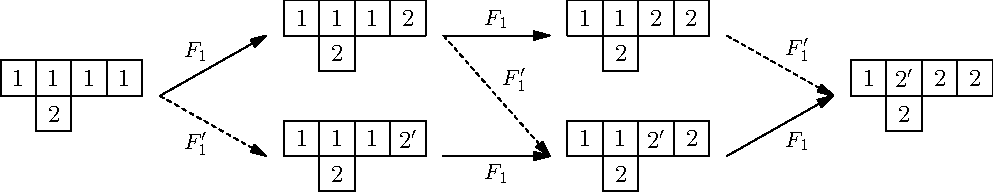
\includegraphics[width=.9\linewidth]{figures/two-row2.pdf} \vspace{1cm}

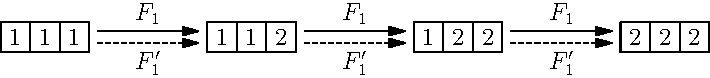
\includegraphics[width=.85\linewidth]{figures/one-row2.pdf}

\caption{\label{fig:two-row}The crystals of the form $\ShST(\lambda,2)$ are ``two-row'' and ``one-row'' diagrams, organizing the tableaux into ``doubled'' crystals. \emph{Above}: the tableaux of shapes $(4,1)$ and $(3)$. Wherever an arrow is missing, the corresponding operator is not defined. Reversing the arrows gives the partial inverses $E_1$ and $E_1'$.} 
\end{figure}
\begin{figure}[htb]\centering
\begin{tabular}{cc}
\setlength{\unitlength}{3em}
\ \ \begin{picture}(5,3)(0,0)
\multiput(0,0)(0,0.2){16}{\line(0,1){0.1}}
\multiput(0,0)(0.2,0){17}{\line(1,0){0.1}}
\put(0,1.2){\circle*{0.1}}
\put(0,1.2){\vector(0,1){.7}\vector(1,0){.7}}
\put(-0.265,1.95){\small{$2$,$2'$}}
\put(0.4,1.3){\small{$1$,$1'$}}
%
\put(1.4,0){\circle*{0.1}}
\put(1.4,0){\vector(0,1){.7}\vector(1,0){.7}}
\put(1.5,0.6){\small{2,2'}}
	\put(2.0,0.1){\small{1,1'}}%
%
\put(2.8,2.2){\circle*{0.1}}
\put(2.8,2.2){\vector(0,1){.7}\vector(1,0){.7}}
\put(2.8,2.2){\vector(0,-1){.7}}
\put(2.8,2.2){\vector(-1,0){.7}}
\put(2.7,2.95){\small{$2$}}
\put(3.5,2.1){\small{$1'$}}
\put(2.7,1.2){\small{$1$}}
\put(1.85,2.1){\small{$2'$}}
\end{picture}
&
\ \
\begin{picture}(3,3)(0,0)
\setlength{\unitlength}{3em}
\stepnorth{2}{%
\stepeast{1}{%
\stepeast{1'}{%
\stepsouthshiftW{1}{%
\stepnorthA{2'}{%
\stepnorthA{2}{%
\stepwestshiftS{2'}{%
\stepeastA{1'}{%
\stepeastA{1'}{%
}}}}}}}}}
\put(0,0){\circle*{0.15}}
\put(3,2){\circle{0.15}}
\multiput(0,0)(0,0.2){15}{\line(0,1){0.1}}
\multiput(0,-0.02)(0.2,0){15}{\line(1,0){0.1}}
\end{picture}
\end{tabular}

\caption{The \emph{lattice walk} of a word $w = w_1 w_2 \cdots w_n \in \{1', 1, 2', 2\}^n$. In the interior of the first quadrant, each letter corresponds to a cardinal direction. Along the axes, primed and unprimed letters behave the same way. \emph{Right:} The walk for $w=211'12'22'1'1'$ ends at the point $(3,2)$.\label{fig:lattice-walk-intro}} \end{figure}
\section{Background and Notation}\label{sec:notation}

\subsection{Strings and words}

Let $w = w_1w_2 \dots w_n$ be a string in symbols\break $\{1',1,2',2,3',3,\ldots\}$. We will normally assume that the first occurrence of $\{i,i'\}$ in $w$ is $i$, for each $i\in \{1,2,3,\ldots\}$. Informally, we adopt the convention that the first $i$ can be treated as $i'$ for the purposes of any rule we state, and if any operation produces a string where the first symbol among $\{i,i'\}$ is $i'$, then we will implicitly change it to $i$. We make this rigorous as follows.

\begin{defi}
Let $w$ be a string in symbols $\{1',1,2',2,3',3,\ldots\}$. The \emph{first $i$ or $i'$} of $w$ is the leftmost entry which is either equal to $i$ or $i'$. The \emph{canonical form} of $w$ is the string formed by replacing the first $i$ or $i'$ (if it exists) with $i$ for all $i\in \{1,2,3,\ldots\}$. We say two strings $w$ and $v$ are \emph{equivalent} if they have the same canonical form; note that this is an equivalence relation.
\end{defi}

\begin{defi}
A \emph{word} is an equivalence class $\hat{w}$ of the strings $v$ equivalent to $w$. If $w$ is in canonical form, we say that $w$ is the \emph{canonical representative} of the word $\hat{w}$. We often call the other words in $\hat{w}$ \emph{representatives} of $\hat{w}$ or of $w$. The \emph{weight} of $w$ is the vector $\wt (w) = (n_1, n_2, \ldots ),$ where $n_i$ is the total number of $(i)$s and $(i')$s in $w$.
\end{defi}

\begin{exam}
The canonical form of the word $1'1'2'112'$ is $11'2112'$. The set of all representatives of $11'2112'$ is $\{1'1'2'112',11'2'112',1'1'2112',11'2112'\}$. Note that the word $11'1$ only has two distinct representatives instead of four.
\end{exam}

Given an operator $A:T\to S$ defined on some subset $T\subseteq S$, we will say $A$ is a \emph{partial operator} on $S$, and write $A : S \to S$. We write $A(s)=\varnothing$ when $A$ is not defined on $s$ (\ie $s\not\in T$). Our raising and lowering operators will be partial operators on words.

\subsection{Shifted tableaux and jeu de taquin}

Recall that a \emph{strict partition} is a strictly-decreasing sequence of positive integers, $\lambda=(\lambda_1 > \cdots > \lambda_k)$. We say that $|\lambda|=\sum \lambda_i$ is the \emph{size} of $\lambda$, and the entries $\lambda_i$ are the \emph{parts} of $\lambda$. The \emph{shifted Young diagram} of $\lambda$ is the partial grid of squares in which the $i$-th row contains $\lambda_i$ boxes and is shifted to the right $i$ steps, as in the example shown below. A \emph{(shifted) skew shape} is a difference $\lambda/\mu$ of two partition diagrams, formed by removing the squares of $\mu$ from the diagram of $\lambda$, if $\mu$ is contained in $\lambda$. 

\begin{center}
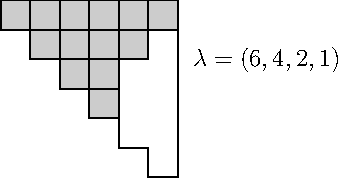
\includegraphics{figures/shifted-partition.pdf} \hspace{1cm}
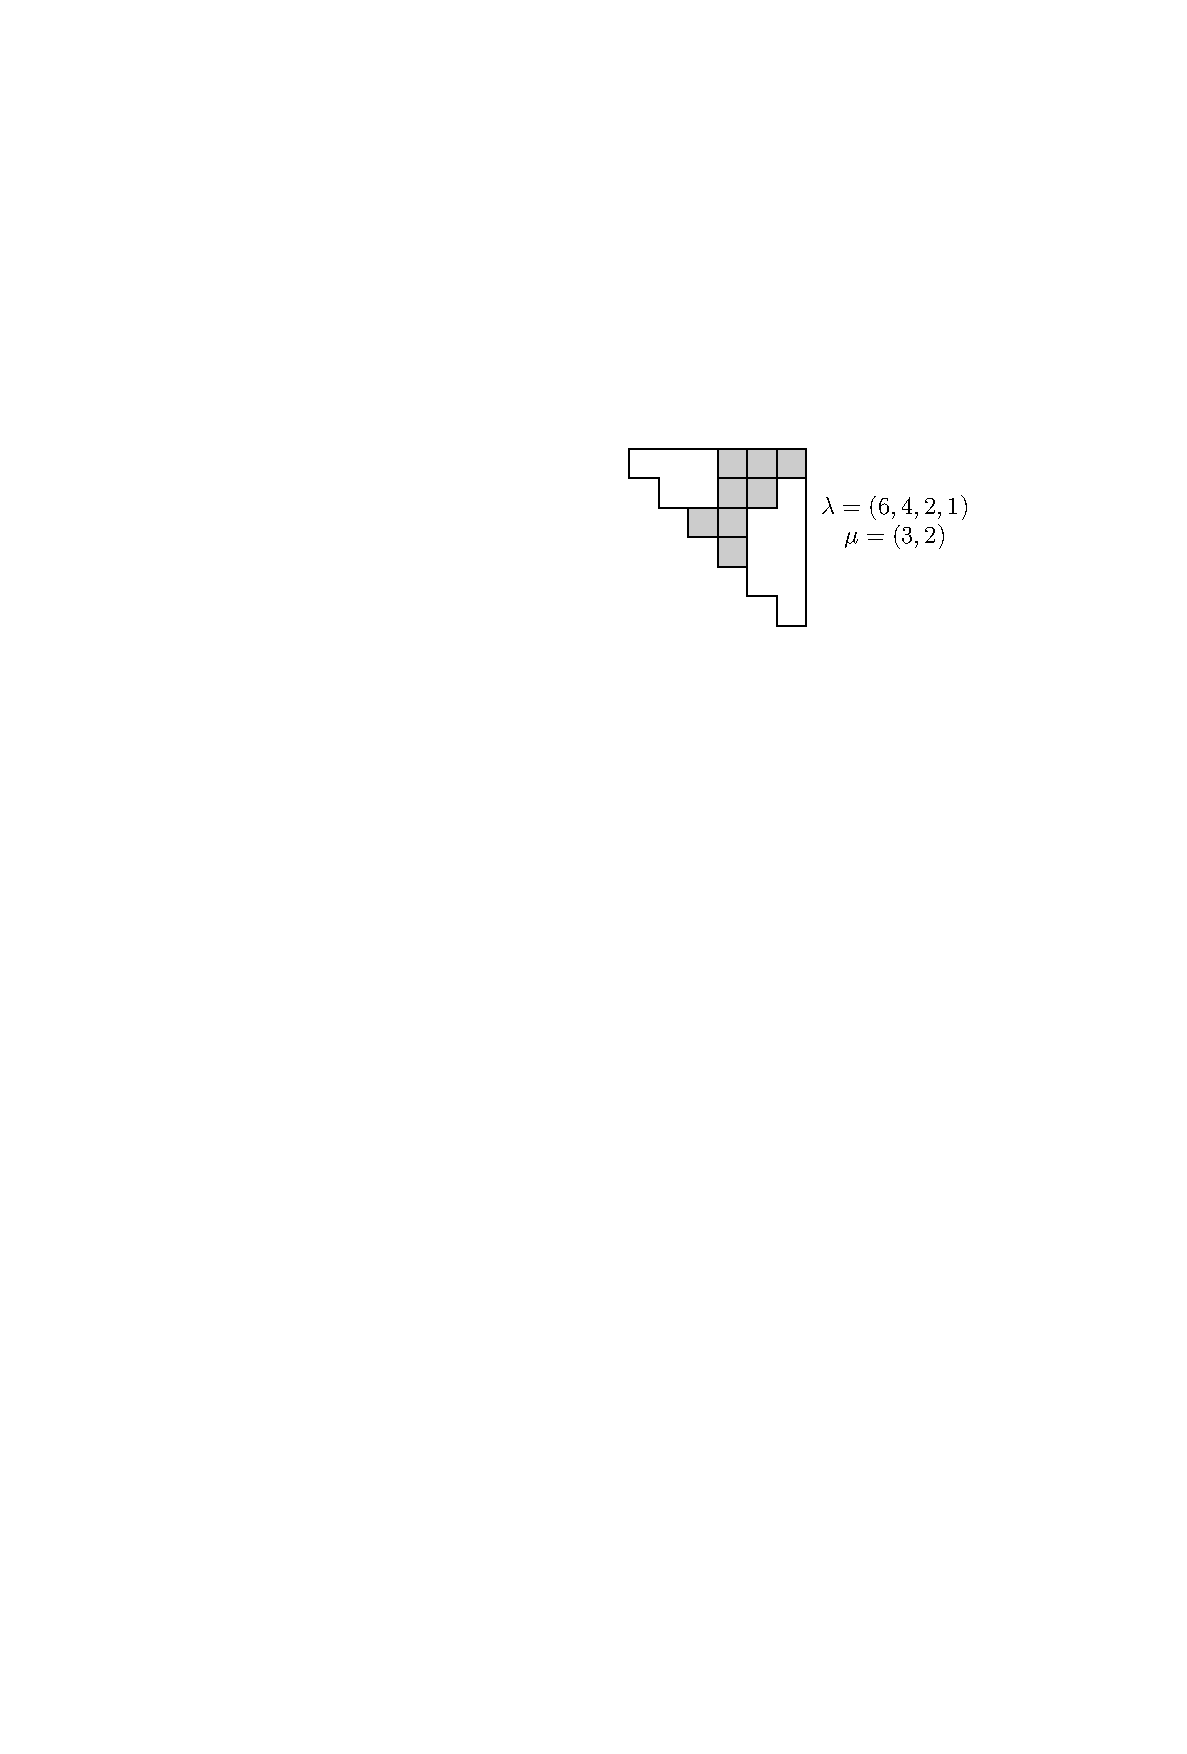
\includegraphics{figures/shifted-partition3.pdf}
\end{center}

A \emph{shifted semistandard Young tableau} is a filling of the boxes with entries from the alphabet $\{1'<1<2'<2<3'<3<\cdots \}$ such that the entries are weakly increasing down columns and across rows, and such that primed entries can only repeat in columns, and unprimed only in rows. The \emph{(row) reading word} of such a tableau is the word formed by concatenating the rows from bottom to top (in the example below, the reading word is $3111'21'12'$). 
The \emph{weight} of $T$ is the vector $\wt (T) = (n_1, n_2, \ldots)$, where $n_i$ is the total number of $(i)$s and $(i')$s in $T$.

\begin{center}
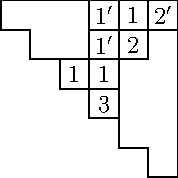
\includegraphics{figures/shifted-semistandard.pdf}
\end{center}

The notion of \emph{jeu de taquin} for shifted tableaux is similar to jeu de taquin for usual tableaux: an \emph{inner jeu de taquin slide} is the process of choosing an empty inner corner of the skew tableau and choosing either the entry to its right or below it to slide into the empty square so as to keep the tableau semistandard, then repeating the process with the new empty square, and so on until the empty square is an outer corner. An \emph{outer jeu de taquin slide} is the reverse process, starting with an outer corner and sliding boxes outwards.

There are two exceptions to the sliding rules: if an outer slide moves an $i$ down into the diagonal and then another $i$ to the right on top of it, that $i$ becomes primed (and vice versa for the corresponding inner slide), as shown below.
\begin{center}
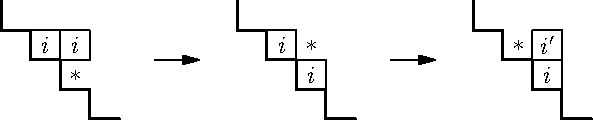
\includegraphics{figures/special-slide.pdf}
\end{center}
Similarly, if an outer slide moves an $i$ down into the diagonal, then moves an $i'$ to the right on top of it, the $i$ becomes primed.
\begin{center}
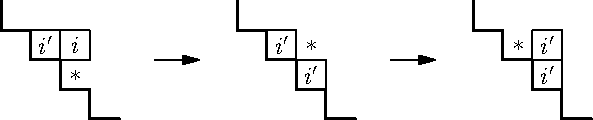
\includegraphics{figures/special-slide-Worley.pdf}
\end{center}

We write $\rectify(T)$ or $\rectify(w)$ to denote the jeu de taquin \emph{rectification} of any shifted semistandard tableau $T$ with reading word $w$; this is well-defined in~\cite{Sagan,Worley}. We say that $T$ is \emph{Littlewood--Richardson}, and $w$ is \emph{ballot}, if for every $i$, the $i$-th row of $\rectify(T)$ consists entirely of $(i)$s.

\begin{defi}
Let $T$ be a semistandard shifted skew tableau with reading word $w$. We say that $T$ is in \emph{canonical form} if $w$ is, and use the same conventions for tableaux as for words: a tableau $T$ in canonical form is identified with the set of \emph{representatives} of $T$, tableaux formed by possibly priming the first $i$ in reading order for each $i$; two tableaux are \emph{equivalent} if they have the same shape and reading their words are equivalent; the set of all representatives of $T$ is the equivalence class of $T$, denoted $\hat T$. 
\end{defi}

We note that switching representatives commutes with jeu de taquin, so instead of working with equivalence classes of tableaux, we will normally assume our tableaux are in canonical form. 

Shifted semistandard tableaux are used to define the Schur $Q$-functions. Equivalence classes of tableaux, on the other hand, arise in formulas involving multiplication of Schur $P$-functions. We elaborate in Section~\ref{sec:characters}. Our motivation for studying crystal strutures is connected to the latter, and so we will be mainly concerned with equivalence classes of tableaux. 

The main property that we wish our operators $E_i$, $E'_i$, $F_i$, $F'_i$ to satisfy is \emph{coplacticity}.

\begin{defi}
An operation on canonical shifted tableaux (or on their reading words) is \emph{coplactic} if it commutes with all shifted jeu de taquin slides.
\end{defi}

\begin{defi}
The \emph{standardization} of a word $w$ is the word $\std(w)$ formed by replacing the letters in order with $1,2,\ldots,n$ from least to greatest, breaking ties by reading order for unprimed entries and by reverse reading order for primed entries. 

The standardization of a shifted tableau $T$ is the standard shifted tableau $\std(T)$ formed by standardizing its reading word and performing the same changes on the corresponding letters of the tableau.
\end{defi}

\begin{exam}
The standardization of the word $1121'22'1'11$ is the word 
$348297156$. Note that this is the same as the standardization of every representative of the word, and in general standardization is well-defined independently of the representative.
\end{exam}

\begin{prop}\label{prop:standardization}
A filling $T$ of a shifted skew shape is semistandard if and only if $\std(T)$ is a standard shifted tableau.
\end{prop}

\begin{proof}
The forward direction is clear. For the reverse direction, suppose $\std(T)$ is a standard shifted tableau. We need to check that any two adjacent entries satisfy the semistandard condition. If $x$ is just left of $y$, then $x<y$ in $\std(T)$. Thus either $x<y$ in $T$ or $x=y$ is unprimed. Similarly, if $x$ is just above $y$ then either $x<y$ in $T$ or $x=y$ is primed. Thus $T$ is semistandard.
\end{proof}

\subsubsection{Shifted dual equivalence}

Two \emph{standard} skew shifted tableaux are said to be (shifted) \emph{dual equivalent} if their shapes transform the same way under any sequence of jeu de taquin slides. (See~\cite{Assaf,Haiman} for more in-depth discussions of dual equivalence.) We extend this notion to \emph{semistandard} shifted tableaux by defining two tableaux to be \emph{dual equivalent} if and only if their standardizations are, as in~\cite{SaganBook}. The word ``dual'' refers to the recording tableau under the shifted Schensted correspondence~\cite{Sagan, Worley}. 

We will occasionally think of a word $w = w_1 \cdots w_n$ as a \defn{diagonally-shaped tableau}, \ie of skew shape $(2n-1, \ldots,3, 1) / (2n-3, \ldots, 1)$. We will say that two words $w, w'$ are dual equivalent if the corresponding diagonal tableaux are dual equivalent.

\subsection{The involutions \texorpdfstring{$\eta_i$}{eta i}}

We will also make use of an important symmetry on words and tableaux, as follows.

\begin{defi}
For a word $w$, we define the word $\eta_i(w)$ by replacing the letters $\{i',i,i{+}1', i{+}1\}$ of any representative of $w$ as follows: we send $i' \mapsto i{+}1$, $i \mapsto i{+}1'$, $i{+}1' \mapsto i$, and $i{+}1 \mapsto i'$. (Note that the choice of representative $v$ of the word $w$ does not affect the output word.)
\end{defi}

\begin{exam} 
We have $\eta_1(121'132) = 2122'31'$.
\end{exam}

It will also be helpful to extend $\eta_i$ to tableaux having only $i',i,i{+}1',i{+}1$ entries. For simplicity we consider $\eta_1$ and the letters $1$ and $2$.

\newcommand{\etaT}{\boldsymbol{\eta}}
\begin{defi}\label{def:eta-on-T}
Let $T$ be a skew shifted tableau in the $n\times n$ staircase with entries in $\{1',1,2',2\}$. Define $\etaT_1(T)$ to be the tableau formed by applying $\eta_1$ to the entries of $T$, reflecting the tableau across the antidiagonal of the $n\times n$ staircase, and reverting to canonical form.
\end{defi}

\begin{center}
\raisebox{-.5\height}{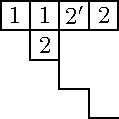
\includegraphics[scale=0.8]{figures/etaT1.pdf}} \qquad $\xrightarrow{\ \eta_1\ }$ \qquad \raisebox{-.5\height}{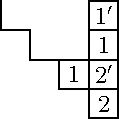
\includegraphics[scale=0.8]{figures/etaT2.pdf}}
\end{center}

To relate this definition back to $\eta_1$ on words, we also define the \emph{column reading word} of a tableau to be the word formed by concatenating the columns from left to right, reading each column from bottom to top.

\begin{rema} \label{rmk:row-col-eta}
It is easy to see that if $w$ is the (row) reading word of $T$ in Definition~\ref{def:eta-on-T} and $v$ is the column reading word of $\etaT_1(T)$, then $v=\eta_1(w)$.
\end{rema}

\begin{rema} \label{rmk:eta-words-dual}
By construction, $\etaT$ is a coplactic operation on tableaux. In particular, two tableaux $T$ and $T'$ are dual equivalent if and only if $\etaT_1(T)$ and $\etaT_1(T')$ are dual equivalent. For words, the situation is similar: $w$ and $w'$ are dual equivalent if and only if $\eta_1(w)$ and $\eta_1(w')$ are dual equivalent (noting that $\etaT_1$ and $\eta_1$ have the same effect on diagonally-shaped tableaux).
\end{rema}


%%%%%%%%%%%%%%%%

\section{The operators \texorpdfstring{$E'$}{E'} and \texorpdfstring{$F'$}{F'}}\label{sec:primed-ops}

Throughout this section, we consider words consisting only of the letters $\{1',1,2',2\}$, and define only the operators $E'_1$ and $F'_1$. For general words $w$, $E'_i$ and $F'_i$ are defined on the subword containing the letters $\{i',i,i{+}1',i{+}1\}$, treating $i$ as $1$ and $i{+}1$ as $2$.

For simplicity we use the following shorthands.

\begin{defi}
Define $E' = E'_1$, $F' = F'_1$, $\eta= \eta_1.$
\end{defi}

To begin, we make the following observation.

\begin{lemma} \label{lem:unstandardize}
Let $s$ be a standard word \textup{(}\ie a permutation of $1, \ldots, n$\textup{)}, and let $n \Mk =\Mk  \sum_{i=1}^k a_i$. There is at most one word $w$ of weight $(a_1,\ldots,a_k)$ and standardization $\std (w) = s$.
\end{lemma}

\begin{proof}
We construct $w$ from $s$. The numbers $1, \ldots, a_1$ of $s$ must become $(1)$s and $(1')$s. Moreover, the assignment of primes is uniquely determined: if $i$ is the first in reading order among $1, \ldots, a_1$, then $1, \ldots, i-1$ must become $(1')$s, and must occur in reverse reading order (or else no such $w$ exists). Similarly, $i, \ldots, a_1$ must become $(1)$s and must occur in reading order. Next, $a_1+1, \ldots, a_1+a_2$ must become $(2)$s and $(2')$s, and the assignment of primes is again (at most) uniquely determined. The argument continues inductively.
\end{proof}

Consequently, the following definition makes sense. Let $\alpha$ be the vector $(1,-1)$ and let $w$ be a word.

\begin{defi}[Primed operators] \label{def:primed-operators}
We define $E'(w)$ to be the unique word such that
\[
\std (E'(w)) = \std (w) \hspace{0.5cm}\text{ and }\hspace{0.5cm} \wt (E'(w)) = \wt (w) + \alpha,
\]
if such a word exists; otherwise, $E'(w) = \varnothing$. We define $F'(w)$ analogously using $-\alpha$.
\end{defi}

The key properties of $E'$ and $F'$ are as follows.

\begin{prop} \label{prop:primed-partial-inverses}
The maps $E'$ and $F'$ are partial inverses of each other, that is, $E'(w) = v$ if and only if $w = F'(v)$.
\end{prop}

\begin{proof}
This is immediate from the definitions of $E'$ and $F'$.
\end{proof}

\begin{prop} \label{prop:primed-eta}
We have $E' = \eta \circ F' \circ \eta$.
\end{prop}

\begin{proof}
Observe that $\eta$ inverts the standardization numbering, sending $i \mapsto n+1-i$, and so $\std (\eta \circ F' \circ \eta(w)) = \std (w)$. Then observe that $\eta$ also reverses the weight.
\end{proof}

\begin{prop} \label{prop:primed-semistandard}
The maps $E'$ and $F'$ preserve semistandardness when defined. That is, if $E'$ \textup{(}\resp $F'$\textup{)} is defined on a skew shifted semistandard tableau $T$, then $E'(T)$ \textup{(}\resp $F'(T)$\textup{)} is semistandard.
\end{prop}


\begin{proof}
Since $E'$ and $F'$ preserve standardization when defined, this follows from Proposition~\ref{prop:standardization}. 
\end{proof}

\begin{prop} \label{prop:primed-coplactic}
The operations $E'$ and $F'$ are coplactic, that is, they commute with all jeu de taquin slides.
\end{prop}

\begin{proof}
The slide path of a jeu de taquin slide on $T$ depends only on $\std (T)$. Hence, if $T' = E'(T)$ or $F'(T)$, applying a jeu de taquin slide gives a new pair of tableaux with the same standardization, and with weight differing by $\pm \alpha$, as desired.
\end{proof}

We also note that the primed operators $F'_i, E'_i$ for \emph{different} $i$ commute when defined:

\begin{prop} \label{prop:primed-operators-commute}
Let $w$ be a word on an arbitrary alphabet $\{1', 1, \ldots, n', n\}$. Then $F'_i F'_j(w) = F'_j F'_i(w)$ whenever both are defined, and likewise for all other pairs from $F'_i, E'_i, F'_j, E'_j$.
\end{prop}

\begin{proof}
This is immediate from the definition, since the effect is to change $\wt (w)$ by the corresponding sum of vectors $\pm \alpha_i$, while preserving $\std (w)$.
\end{proof}


We now describe the action of $E'$ and $F'$ in a computationally convenient way.

\begin{prop}\label{prop:explicit-definitions-primed}
If $\wt(w)_1>0$ and there exists a representative $u$ of $w$ in which there is no $2'$ after the last $1$, then $F'(w)$ is obtained by changing the last $1$ to a $2'$ in~$u$. Otherwise $F'(w) = \varnothing$. 

The word $E'(w)$ is defined similarly with the roles of $1$ and $2'$ reversed: if $\wt(w)_2>0$ and there is no $1$ after the last $2'$ in some representative $u$, change the last $2'$ to a~$1$ in $u$. Otherwise $E'(w) = \varnothing$.
\end{prop}

\begin{proof}
Since $F'$ is the unique operator that preserves standardization and lowers the weight, say from $(a,b)$ to $(a-1,b+1)$, we see from the construction in the proof of Lemma~\ref{lem:unstandardize} that the entry that changes weight is precisely the entry that standardizes to $a$. This is the last $1$ in reading order, and changing it to a $2'$ is the only potential way to preserve standardization. In order for it to do so, it must also be to the right of the last $2'$ in reading order (under any possible representative).

The analysis is similar for $E'$.
\end{proof}

\begin{rema}
In Proposition~\ref{prop:explicit-definitions-primed}, if $F'(w)$ is defined then it is in fact defined on the canonical representative. However, this is not the case for $E'$. For instance, if $w=1121'22$ then there is no $2'$ in the canonical form, but in the representative $112'1'22$ the last $2'$ is to the right of the last $1$, and $E'(w)=1111'22$. 

As another example, if $v=22'11'$, then in canonical form the last $2'$ is to the left of the last $1$, but in the representative $22'1'1'$ it is not as there is no $1$. In this case we have $E'(v)=211'1'$, and the canonical forms of $v$ and $E'(v)$ differ by two letters, not one.
\end{rema}


This also allows us to describe the action on straight shifted tableaux $T$.

\begin{prop} \label{prop:rect-primed-action}
If $T$ has one row, $E'(T)$ \textup{(}respectively $F'(T)$\textup{)} is obtained by changing the leftmost $2$ to a $1$ \textup{(}respectively, the rightmost $1$ to a $2$\textup{)}, if possible; otherwise it is $\varnothing$.

If $T$ has two rows and its first row contains a $2'$, then $E'(T)$ is obtained by changing the $2'$ to a $1$, and $F'(T) = \varnothing$. If the first row does not contain a $2'$, $E'(T) = \varnothing$ and $F'(T)$ is obtained by changing the rightmost $1$ to a $2'$.
\end{prop}

\begin{exam} Here are some maximal chains for $F'$:
\begin{gather*}
12211' \xrightarrow{F'} 1222'1' \xrightarrow{F'} \varnothing
\\
1111'1' 
\xrightarrow{F'} 1121'1' 
\xrightarrow{F'} 1221'1' 
\xrightarrow{F'} 22211' 
\xrightarrow{F'} 2222'1
\xrightarrow{F'} 2222'2'
\xrightarrow{F'} \varnothing
\end{gather*}
\end{exam}


We conclude this section with a note on the lengths of chains in the primed operators. The maximal chains for $F'$ will normally have length $1$ (as in the first example above). We get longer chains (as in the second example above) if and only if $\rectify(w)$ has only one row. 

\begin{prop}\label{lem:maxchains}
A maximal chain for $F'$ has length greater than $1$ if and only if $\rectify(w)$ has one row \textup{(}and at least two boxes\textup{)}. Moreover, when $\rectify(w)$ has two rows, $F'(w) = \varnothing$ iff $E'(w) \neq \varnothing$ iff $\rectify(w)$ contains a $2'$ in its first row.
\end{prop}

\begin{proof}
By coplacticity, it suffices to show this for the reading word of a straight shifted tableau. Then we apply the previous Proposition. \end{proof}


\section{The lattice walk of a word}\label{sec:walks}

\looseness-1
The first step in defining the more involved operators $F(w)$ and $E(w)$ is to associate, to each word $w$, a lattice walk in the first quadrant of the plane. This walk is a sequence 
\[
P_0(w), P_1(w), \ldots, P_n(w)
\]
 of points in $\NN \times \NN$, starting with $P_0(w) = (0,0)$. We specify the walk by assigning a step to each $w_i$, $i=1, \dots, n$; any choice of representative of $w$ will give the same walk. Each step will be one of the four principal direction vectors:
\[
\east{~~} \ =\ (1,0)
\qquad \west{~~} \ =\ (-1,0)
\qquad \north{} \ =\ (0,1)
\qquad \south{} \ =\ (0,-1)\,.
\]
$P_i(w)$ is (as usual) the sum of the steps assigned to $w_1, \dots, w_i$. We define the walk inductively, as follows. Suppose $i >0$, and we have assigned steps to $w_1, \dots, w_{i-1}$, so $P_0(w), \dots,P_{i-1}(w)$ have been defined. Write $P_{i-1}(w) = (x_{i-1},y_{i-1})$. We assign the step to $w_i$ according to
Figure~\ref{fig:directions}, with two cases based on whether or not the step starts on one of the $x$ or $y$ axes. See Figure~\ref{fig:lattice-walk-intro}. We will generally write the label each step of the walk by the letter $w_i$, so as to represent both the word and its walk on the same diagram.


\begin{figure}[htb]\centering
\begin{tabular}{|c|cccc|}
\hline
$x_iy_i=0$ & \east{1'} & \east{1} & \north{2'} & \north{2} \\[.8ex]
\hline
$x_iy_i\neq0$ &\east{1'} & \south{1} & \west{2'} & \north{2} \\[.8ex]
\hline
\end{tabular}

\caption{\label{fig:directions} The directions assigned to each of the letters $w_i=1'$, $1$, $2'$, or $2$ according to whether the location of the walk just before $w_i$ starts on the axes ($x_iy_i=0$) or not.}
\end{figure}



\begin{exam}
\label{ex:walk}
Here is the walk for $w = 1221'1'111'1'2'2222'2'11'1$.

\begin{center}
\begin{picture}(5,4.8)(0,-0.2)
%\begin{picture}(5,4.2)(0,0)
\multiput(0,0)(0,0.2){22}{\line(0,1){0.1}}
\multiput(0,0)(0.2,0){27}{\line(1,0){0.1}}
\put(0,0){\circle*{0.13}}
\put(4,2){\circle{0.13}}
\stepeast{1}{%
\stepnorth{2}{%
 \stepnorth{2}{%
\stepeast{1'}{%
\stepeast{1'}{%
\stepsouth{1}{%
\stepsouth{1}{%
\stepeast{1'}{%
\stepeast{1'}{%
\stepnorth{2'}{%
\stepnorth{2}{%
\stepnorth{2}{%
\stepnorth{2}{%
\stepwest{2'}{%
\stepwest{2'}{%
\stepsouth{1}{%
\stepeast{1'}{%
\stepsouth{1}{%
}}}}}}}}}}}}}}}}}}
\end{picture}
\end{center}
\end{exam}



\begin{prop}
The walk for $\eta(w)$ is the reflection of the walk for $w$ over the line $y=x$.
\end{prop}

\begin{proof}
This is clear by the symmetry of the lattice walk operations.
\end{proof}

The key property of this lattice walk is that its length, $n$, and its endpoint, $P_n(w) = (x_n, y_n)$, tell us almost everything about the rectification tableau $\rectify(w)$. Note that $\rectify(w)$ is a straight shifted tableau with at most two rows.

\begin{theorem}\label{thm:rectification}
The shape of $\rectify(w)$ is $\lambda = (\lambda_1, \lambda_2)$, where
\begin{align*}
\lambda_1 &= \tfrac{1}{2}(n+x_n+y_n) = \#\big\{\ \north{} \text{ and/or } \east{} \text{ steps in the walk\ }\big\}, \\
\lambda_2 &= \tfrac{1}{2}(n-x_n-y_n) = \#\big\{\west{} \text{ and/or } \south{} \text{ steps in the walk\ }\big\},
\end{align*}
Moreover, there are $\tfrac{1}{2}(n+x_n-y_n)$ $(1)$s in the first row; there is at most one $2'$, and the remaining entries in the tableau are all $(2)$s.
\end{theorem}

\begin{coro}
The shape of $\rectify(w)$ has only one row iff all
steps in the walk are $\east{~}$ or $\north{}$.
\end{coro}

As an additional corollary, we obtain a new criterion for ballotness:

\begin{coro} \label{cor:ballot-walk-criterion}
A word $w$ is ballot if and only if for all $i$, the lattice walk of the subword $w_i$ consisting of the letters $i,i',i+1,i+1'$ has $y_n = 0$, that is, ends on the $x$-axis. Similarly $w$ is anti-ballot \textup{(}\ie $\eta(w)$ is a ballot word\textup{)} if and only if $x_n = 0$ for all $i$.
\end{coro}

\begin{proof}
It is well-known that a word is ballot if and only if each subword $w_i$ is ballot (see~\cite{Stembridge}, for instance). By definition, $w_i$ is ballot if and only if the first row of $\rectify(w_i)$ consists only of $(1)$s (after replacing $i',i \leadsto 1',1$ and $i+1',(i+1) \leadsto 2',2$). By Theorem~\ref{thm:rectification}, this says $\tfrac{1}{2}(n+x_n-y_n) = \tfrac{1}{2}(n+x_n+y_n)$, that is, $y_n=0$.
\end{proof}


Our proof uses the rules of shifted Knuth equivalence, as developed in~\cite{Sagan} and~\cite{Worley}. Using our primed notation, their shifted Knuth moves are as follows.

\begin{defi}
Two words $w$ and $v$ are \emph{shifted Knuth equivalent} if they differ by a sequence of elementary shifted Knuth moves on adjacent letters, consisting of either:
\begin{itemize}
\item $bac\leftrightarrow bca$ where under the standardization ordering we have $a<b<c$,
\item $acb\leftrightarrow cab$ where under the standardization ordering we have $a<b<c$,
\item Interchanging the first two letters at the start of the word,
\item If the first two letters in the word are unprimed and equal, priming the second; or, if the first two letters are $aa'$, un-priming the second.
\end{itemize}
In the moves $bac \leftrightarrow bca$ and $acb \leftrightarrow cab$, we call $b$ the \emph{pivot} and $a,c$ the \emph{switched pair}.
\end{defi}

\begin{exam}
Note that $2'12'\to 12'2'$ is a valid elementary shifted Knuth move of the second type above, since under the standardization ordering the right-hand $2'$ is less than the other $2'$. On the other hand $212\to 122$ is not valid, because the right-hand $2$ is considered greater than the other $2$.
\end{exam}

Sagan and Worley (\cite{Sagan}, \cite{Worley}), in slightly different notation, showed that shifted Knuth equivalence classes on words are in one-to-one correspondence with semistandard shifted straight shape tableaux, via either JDT rectification or mixed insertion. We will show that the walk's endpoint is an invariant of the equivalence class.

\begin{prop}\label{prop:walks}
The endpoint of the lattice walk of a word $w$ is invariant under all shifted Knuth moves.
\end{prop}
It will then suffice to check Theorem~\ref{thm:rectification} on words of rectified tableaux. 

\begin{proof}
The first two steps of the walk always lie on the axes, so those steps follow the rules for $xy = 0$, regardless of which letters occur. Thus from now on we assume the switched pair are not the first two letters of the word; in particular, upon reaching the pair, the walk's location is not the origin.

Let $a,c$ be the switched pair; let $(x,y)$ be the location of the walk just before the switched pair, and let $b$ be th²e pivot. We show that the endpoint of the triple is preserved. Note that, for any such triple, it suffices to show that the directions of the arrows of the switched pair are unchanged, and in most cases below (but not all) this will hold.

Note that applying $\eta$ has the effect of reversing the standardization numbering (and transposing the walk and its endpoint). In particular, $\eta$ takes Knuth moves to Knuth moves. We use this symmetry to reduce the number of cases to consider.

\begin{enonce*}[remark]{Case 1} $\{a,c\} = \{1',2\}$. There is nothing to check because the directions of $1'$ and $2$ arrows never change.
\end{enonce*}

\begin{enonce*}[remark]{Case 2} $\{a,c\} = \{2',2\}$ or $\{1',1\}$. By applying $\eta$, it suffices to consider $\{2',2\}$, say $a=2'$ and $c=2$, and to show that the $a=2'$ arrow does not change directions after the switch. The standardization order forces the pivot to be on the left (\ie the exchange is $bca \leftrightarrow bac$) and to be $b = 2'$ or $2$; in particular $y>0$. If $x=0$, then $a=2'$ contributes $\north{}$ in both cases; if instead $x>0$, then in both cases $a=2'$ occurs off the axes, hence gives $\west{}$.
\end{enonce*}

\begin{enonce*}[remark]{Case 3} $\{a,c\} = \{1,2\}$ or $\{1',2'\}$. By applying $\eta$, it suffices to consider $\{1,2\}$. If the pivot is on the left, then it must be $2'$ or $2$, so again $y>0$ and the reasoning is exactly as in Case 2 but for $a=1$ rather than $a=2'$. If the pivot is on the right, then it is $b=1$ or $2'$, and we show that the location of the walk just before $b$ is unchanged under $acb\leftrightarrow cab$. If $y>0$, the arrow $a=1$ is $\south{}$ in both cases. If instead $y=0$ (and so $x \ne 0$ since the location is not the origin), the individual steps change; see Figure~\ref{fig:knuthmove-switch12} for the remaining possibilities. 

\begin{figure}[htb]\centering
%\begin{picture}(1,1)(0,0.4)
\begin{picture}(1,1.5)(0,0.0)
\multiput(-0.2,0)(0.2,0){8}{\line(1,0){0.1}}
\put(0,0){\circle*{0.2}}
\put(1,0){\circle{0.2}}
\stepnorth{2}{%
\stepsouthshiftE{1}{%
\stepeast{1}}}
\end{picture}
$\longsquiggly$
%\begin{picture}(1,1)(0,0.4)
\begin{picture}(1,1.5)(0,0.0)
\multiput(-0.2,0)(0.2,0){8}{\line(1,0){0.1}}
\put(0,0){\circle*{0.2}}
\put(1,0){\circle{0.2}}
\stepeast{1}{%
\stepnorthshiftW{2}{%
\stepsouth{1}}}
\end{picture}
\hspace{2cm}
%\begin{picture}(1,1)(0,0.4)
\begin{picture}(1,1.5)(0,0.0)
\multiput(-0.2,0)(0.2,0){6}{\line(1,0){0.1}}
\put(0,0){\circle*{0.2}}
\put(0,1){\circle{0.2}}
\stepnorthshiftW{2}{%
\stepsouth{\ 1,2'}{%
\put(0.1,0){\rlap{\stepnorth{}}}
}}
\end{picture}
$\longsquiggly$
%\begin{picture}(1,1)(0,0.4)
\begin{picture}(1,1.5)(0,0.0)
\multiput(-0.2,0)(0.2,0){8}{\line(1,0){0.1}}
\put(0,0){\circle*{0.2}}
\put(0,1){\circle{0.2}}
\stepeast{1}{%
\stepnorth{2}{%
\stepwest{2'}}}
\end{picture}

\caption{The unique Knuth moves where switching a $1,2$ pair alters the individual steps of the walk. In both cases, the walk begins with $x>0, y=0$. \emph{Left}: The move $211 \leftrightarrow 121$. \emph{Right}: The move
$212' \leftrightarrow 122'$.}
\label{fig:knuthmove-switch12}
\end{figure}
\end{enonce*}

\begin{enonce*}[remark]{Case 4} $\{a,c\} = \{1,2'\}$. The standardization order forces the pivot to be on the right, and it must be $b = 1$ or $2'$. By applying $\eta$, we may assume $b=1$. If $x>1$ and $y>1$, both $a,c$ steps occur off the axes, so we're done; otherwise the path changes in five different ways depending on whether $x,y$ are variously $0$ or $1$ (see Figure~\ref{fig:knuthmove-switch12'}).\qedhere 
\end{enonce*}

\end{proof}

\begin{figure}[htb]\centering

$x=0, y\geq 1$: \hspace{0.1cm} 
\begin{picture}(1,1)(0,0.4)
\multiput(0,-0.2)(0,0.2){7}{\line(0,1){0.1}}
\put(0,0){\circle*{0.2}}
\put(1,0){\circle{0.2}}
\put(0.20,0.23){\scriptsize{$1,2',1$}}
\put(0,-0.1){\stepeast{}{%
\put(0,0.1){\stepwest{}{%
\put(0,0.1){\stepeast{}}}}}}
\end{picture}
\hspace{0.3cm}$\longsquiggly$\hspace{0.3cm}
\begin{picture}(1,1)(0,0.4)
\multiput(-0.03,-0.2)(0,0.2){7}{\line(0,1){0.1}}
\put(0,0){\circle*{0.2}}
\put(1,0){\circle{0.2}}
\put(-0.3,0.4){\scriptsize{2'}}
\stepnorth{}{%
\stepeast{1}{%
\put(0,0){\stepsouth{1}}%
}}
\end{picture}
\vspace{1cm} \\
 $x\geq 1, y=0$: \hspace{0.1cm}
\begin{picture}(1,1)(0,0.4)
\multiput(-0.2,0)(0.2,0){8}{\line(1,0){0.1}}
\put(0,0){\circle*{0.2}}
\put(1,0){\circle{0.2}}
\stepeast{1}{%
\stepnorthshiftW{2'}{%
\stepsouth{1}}}
\end{picture}
\hspace{0.5cm}$\longsquiggly$\hspace{0.5cm}
\begin{picture}(1,1)(0,0.4)
\multiput(-0.2,0)(0.2,0){8}{\line(1,0){0.1}}
\put(0,0){\circle*{0.2}}
\put(1,0){\circle{0.2}}
\stepnorth{2'}{%
\stepsouthshiftE{1}{%
\stepeast{1}}}
\end{picture}
\vspace{1cm} \\ 
$x=1,y>1$: \hspace{0.2cm}
\begin{picture}(1,1)(-1,-0.6)
\multiput(-1,-1.2)(0,0.2){7}{\line(0,1){0.1}}
\put(0,0){\circle*{0.2}}
\put(0,-1){\circle{0.2}}
\stepsouth{1}{%
\stepwestshiftN{2'}{%
\stepeast{1}}}
\end{picture}
\hspace{0.3cm}$\longsquiggly$\hspace{0.3cm}
\begin{picture}(1,1)(-1,-0.6)
\multiput(-1,-1.2)(0,0.2){7}{\line(0,1){0.1}}
\put(0,0){\circle*{0.2}}
\put(0,-1){\circle{0.2}}
\stepwest{2'}{%
\stepeastshiftS{1}{%
\rlap{\stepsouth{1}}
}}
\end{picture}
\vspace{1cm} \\
$x>1,y=1$: \hspace{0.2cm} 
\begin{picture}(1,1)(0,-0.6)
\multiput(-0.3,-1)(0.2,0){7}{\line(1,0){0.1}}
\put(0,0){\circle*{0.2}}
\put(0,-1){\circle{0.2}}
\put(-0.1,0){\stepsouth{}{%
\put(0.1,0){\stepnorth{}{%
\put(0.1,0){\rlap{\stepsouth{1,2',1}}}}}}}
\end{picture}
\hspace{0.1cm}$\longsquiggly$\hspace{1cm}
\begin{picture}(1,1)(0,-0.6)
\multiput(-1.2,-1)(0.2,0){8}{\line(1,0){0.1}}
\put(0,0){\circle*{0.2}}
\put(0,-1){\circle{0.2}}
\stepwest{2'}{%
\stepsouth{1}{%
\stepeast{1}}}
\end{picture}
\vspace{1cm} \\
\hspace{0.5cm} $(x,y) = (1,1)$:\hspace{1.2cm} 
\begin{picture}(1,1)(0,-0.6)
\multiput(-1,-1.2)(0,0.2){7}{\line(0,1){0.1}}
\multiput(-1.2,-1)(0.2,0){8}{\line(1,0){0.1}}
\put(0,0){\circle*{0.2}}
\put(0,-1){\circle{0.2}}
\put(-0.1,0){\stepsouth{}{%
\put(0.1,0){\stepnorth{}{%
\put(0.1,0){\rlap{\stepsouth{1,2',1}}}}}}}
\end{picture}
\hspace{0.1cm}$\longsquiggly$\hspace{1cm}
\begin{picture}(1,1)(0,-0.6)
\multiput(-1,-1.2)(0,0.2){7}{\line(0,1){0.1}}
\multiput(-1.2,-1)(0.2,0){8}{\line(1,0){0.1}}
\put(0,0){\circle*{0.2}}
\put(0,-1){\circle{0.2}}
\stepwest{2'}{%
\stepeastshiftS{1}{%
\rlap{\stepsouth{1}}}}
\end{picture}

\caption{Effects\vrule height 15pt depth 0pt width0pt\ on the walk of the Knuth move $12'1 \leftrightarrow 2'11$. There are five cases in which the individual steps change; the starting point $\bullet$ must have at least one coordinate equal to $1$ or $0$ (but is assumed not be $(0,0)$).}
\label{fig:knuthmove-switch12'}
\end{figure}


\begin{proof}[Proof of Theorem~\ref{thm:rectification}]
By Proposition~\ref{prop:walks}, it suffices to check the statement for words of straight shifted tableaux. In particular, $w$ has the form $2^a 1^a w'$, where $w' = 1^b (2')2^*$, and the $2'$ is optional unless $b=0$, in which case it is required. Let $c$ be the number of $2'/2$s in this suffix, so that $n = 2a + b + c$ and the shape of the tableau is $(a+b+c,a)$. Unwinding the desired statements, we wish to show that the endpoint is $(b,c)$.

If $a=0$, the walk simply moves $b$ steps right and $c$ steps up. If $a>0$, the $2^a1^a$ prefix consists of $a$ steps $\north{}$, one step $\east{}$ and $a-1$ steps $\south{}$, ending at $(1,1)$. Then, if $b>0$, the walk moves down and along the $x$-axis to $(b,0)$, then up for the remaining $2'$ and/or $2$ steps to $(b,c)$. If instead $b=0$, the suffix is just $w' = 2'2^{c-1}$, so the walk moves left and up the $y$-axis, ending at $(0,c)$. In all cases the endpoint is $(b,c)$ as desired.
\end{proof}

Finally, we compute the effects of $E',F'$ on the endpoint of the lattice walk.

\begin{prop} \label{prop:primed-lattice-endpoint}
Applying $F'$ changes precisely one step of the lattice walk, either from $\east{}$ to $\north{}$ or from $\south{}$ to $\west{}$. Consequently, it shifts the endpoint by $(-1,+1)$. For $E'$, the action is reversed.
\end{prop}

\begin{proof}
Since $F'$ and $E'$ are partial inverses, it suffices to prove the statement about $F'$. Consider a representative of $w$ in which the last $1$ is to the right of the last $2'$, and suppose this $1$ is the $i$-th letter, $w_i$. Then by Proposition~\ref{prop:explicit-definitions-primed}, $F'(w)$ is formed by changing $w_i$ to $2'$ and canonicalizing. 

The first $i-1$ steps of the walk are unchanged (since canonicalization does not change the direction of any arrow and nothing else changed), and the arrow $w_i$ changes as stated depending on whether it is on an axis. Finally, because $w_i$ is the last $1$ and is to the right of the last $2'$, every letter after $w_i$ is either $1'$ or $2$, so the later steps' directions are unchanged as well.
\end{proof}

Finally, we show that, despite the special rules governing the axes, the shape of a walk does not change drastically if we shift its start point:

\begin{prop}[Bounded error] \label{lem:bounded-error}
Let $w$ be a word; consider the walk for $w$ beginning at an arbitrary starting point $(x_0,y_0)$, not necessarily the origin. 

\looseness-1
If we shift the start by either $\west{}$ or $\north{}$, then the endpoint also shifts by \emph{either} $\west{}$ or $\north{}$.

\looseness-1
Similarly, if we shift the start by $\east{}$ or $\south{}$, the endpoint also shifts by $\emph{either}$ $\east{}$ or~$\south{}$.
\end{prop}

\begin{proof}
\looseness-1
We prove the first statement; the second follows by applying $\eta$. Working inductively, it suffices to show that, for a single letter $a \in \{1',1,2',2\}$, if we shift its starting point by either $\west{}$ or $\north{}$, then its endpoint also shifts by either $\west{}$ or $\north{}$. This is clear if $a = 1'$ or $2$, or if the shift does not move the starting point on or off the axes.

We check the other cases. If we shift the starting point of $a$ by $\north{}$ off of the $x$-axis (and we are not on the $y$-axis), we see for both $a = 1,2'$ that the endpoint shifts overall by $\west{}$: 
\begin{center}
\begin{picture}(0,1)(0,0)
\put(0,1){\circle{0.2}}
\multiput(-0.3,0)(0.2,0){4}{\line(1,0){0.1}}
\put(0.45,0.4){$\leadsto$}
\stepnorth{2'}{}
\end{picture}
\hspace{2cm}
\begin{picture}(0,0.5)(0,-1)
\multiput(-0.3,-1)(0.2,0){4}{\line(1,0){0.1}}
\put(-1,0){\circle{0.2}}
\stepwest{2'}{}
\end{picture}
\hspace{2cm}
\begin{picture}(0,1)(0,0)
\multiput(-0.3,0)(0.2,0){4}{\line(1,0){0.1}}
\put(1,0){\circle{0.2}}
\put(1.3,0.4){$\leadsto$}
\stepeast{1}{}
\end{picture}
\hspace{2cm}
\begin{picture}(0,0.5)(0,-1)
\multiput(-0.3,-1)(0.2,0){4}{\line(1,0){0.1}}
\put(0,-1){\circle{0.2}}
\stepsouth{1}{}
\end{picture}
\end{center}
Similarly, if $a$ moves $\west{}$ onto the $y$-axis (and was not already on the $x$-axis), in both cases $a = 1,2'$ the endpoint shifts (overall) by $\north{}$.
\end{proof}

\begin{coro} 
\label{cor:concat-ballot}
A concatenation of ballot words is ballot.
\end{coro}
\begin{proof}
Suppose $w_1, w_2$ are ballot, and let $(x_1,0)$, $(x_2,0)$ be the endpoints of their lattice walks. Then, in the lattice walk for $w_1w_2$, the $w_2$ portion begins at $(x_1,0)$ rather than the origin. By Proposition~\ref{lem:bounded-error}, its new endpoint moves $x_1$ steps down and/or right, but clearly can only move right. Thus the endpoint of $w_1w_2$ is at $(x_1+x_2,0)$.
\end{proof}

%%%%%%%%%%%%%%%%
\section{The operators \texorpdfstring{$E$}{E} and \texorpdfstring{$F$}{F}}\label{sec:unprimed-ops}

As in the previous section, throughout this section we assume that $w$ is a word consisting only of letters from $\{1',1,2',2\}$, and for simplicity we use the following notation.

\begin{defi}
Define $E=E_1$, $F=F_1$ and $\eta = \eta_1$.
\end{defi}

There are several parts to this section: we first define $E$ and $F$ and show that they are partial inverses, then prove the main theorem (that $E$ and $F$ are coplactic) in several steps. We show that the operators preserve semistandardness; we then show that they preserve the dual equivalence class of $T$, and finally that they are coplactic.

%%%%%%%%%%%%%%%%
\subsection{Critical substrings and definition of \texorpdfstring{$E$}{E} and \texorpdfstring{$F$}{F}}\label{sec:EFdefinition}

\begin{defi}
If $w$ is a word and $u = w_k w_{k+1} \dots w_l$ is a substring of some representative of $w$, we say $u$ is a \emph{substring} of the word $w$. We say $(x,y) = P_{k-1}(w)$ is the \defn{location} of $u$.
\end{defi}

\begin{defi} We say that $u$ is an \defn{$F$-critical substring} if certain conditions on $u$ and its location are met. There are five types of $F$-critical substring. Each row of the first table in Figure~\ref{fig:criticals} describes one type, and a transformation that can be performed on that type.

%
For example, the first row indicates that $u$ is a critical substring of type 1F if $u$ is of the form $1(1')^*2'$ and the location $(x,y)$ satisfies $y=0$ or $y=1,\, x \geq 1$. The ``steps'' column shows, in each case, what the direction of the corresponding steps in the walk must be. This is redundant information, as it can be deduced from the ``substring'' and ``location'' conditions; we include it because it is useful for reference.

\end{defi} 

\begin{figure}[htb]\centering
\begin{tabular}{|c|c|c|c|c|}
\hline
\multirow{2}{*}{Type} 
& \multicolumn{3}{c|}{Conditions} & \multirow{2}{*}{Transformation} \\
& \multicolumn{1}{c}{Substring}& \multicolumn{1}{c}{Steps} & Location & 
\\\hline
\hline
\multirow{2}{*}{1F} & 
\multirow{2}{*}{$u = 1(1')^*2'$} &
\east{1} ~ \east{1'} ~ \north{2'} & 
$y=0$ & 
\multirow{2}{*}{$u \to 2'(1')^*2$} \\[.5ex]\cline{3-4}
& & 
\south{1} ~ \east{1'} ~ \north{2'} & 
$y=1$, $x \geq 1$ & 
\\[.5ex]\hline
\multirow{2}{*}{2F} &
\multirow{2}{*}{$u = 1(2)^*1'$} &
\east{1} ~ \north{2} ~ \east{1'} & 
$x = 0$ & 
\multirow{2}{*}{$u \to 2'(2)^*1$} \\[.5ex]\cline{3-4}
&& 
\south{1} ~ \north{2} ~ \east{1'} &
$x = 1$, $y \geq 1$ & 
\\[.5ex]\hline
3F & $u = 1$ & 
\east{1} & 
$y = 0$ & 
$u \to 2$ 
\\\hline
4F & 
$u = 1'$ & 
\east{1'} & 
$x = 0$ & 
$u \to 2'$ 
\\\hline
\multirow{2}{*}{5F} & $u = 1$ 
& \south{1}
& \multirow{2}{*}{$x=1$, $y \geq 1$} 
&
\multirow{2}{*}{undefined} \\[.5ex]\cline{2-3}
& $u=2'$ & \west{2'} &&
\\\hline
\end{tabular}
\vspace{0.5cm}

\begin{tabular}{|c|c|c|c|c|}
\hline
\multirow{2}{*}{Type} 
& \multicolumn{3}{c|}{Conditions} & \multirow{2}{*}{Transformation} \\
& \multicolumn{1}{c}{Substring}& \multicolumn{1}{c}{Steps} & Location & 
\\\hline
\hline
\multirow{2}{*}{1E} & 
\multirow{2}{*}{$u = 2'(2)^*1$} &
\north{2'} ~ \north{2} ~ \east{1} & 
$x=0$ & 
\multirow{2}{*}{$u \to 1(2)^*1'$} \\[.5ex]\cline{3-4}
& & 
\west{2'} ~ \north{2} ~ \east{1} & 
$x=1$, $y \geq 1$ & 
\\[.5ex]\hline
\multirow{2}{*}{2E} &
\multirow{2}{*}{$u = 2'(1')^*2$} &
\north{2'} ~ \east{1'} ~ \north{2} & 
$y = 0$ & 
\multirow{2}{*}{$u \to 1(1')^*2'$} \\[.5ex]\cline{3-4}
&& 
\west{2'} ~ \east{1'} ~ \north{2} &
$y = 1$, $x \geq 1$ & 
\\[.5ex]\hline
3E & $u = 2'$ & 
\north{2'} & 
$x = 0$ & 
$u \to 1'$ 
\\[.5ex]\hline
4E & 
$u = 2$ & 
\north{2} & 
$y = 0$ & 
$u \to 1$ 
\\[.5ex]\hline
\multirow{2}{*}{5E} & $u = 1$ 
& \south{1}
& \multirow{2}{*}{$y=1$, $x \geq 1$} 
&
\multirow{2}{*}{undefined} \\[.5ex]\cline{2-3}
& $u=2'$ & \west{2'} &&
\\\hline
\end{tabular}

\caption{\label{fig:criticals} Above, the table of $F$-critical substrings and their transformations. Below, the table of $E$-critical substrings and their transformations. Here $a(b)^*c$ means any string of the form $abb \dots bc$, including $ac$, $abc$, $abbc$, \etc}
\end{figure}


\begin{rema} All the conditions on the starting location are on the lines $y=0$, $y=1$, $x=0$, or $x=1$. Critical substrings can only occur when the walk touches one of these four lines, which corresponds to the initial subword $w_1w_2 \dots w_{k-1}$ being either ballot, anti-ballot, or close to one of these. (See Figure~\ref{fig:criticals}.)
\end{rema}

We define (by abuse of notation) the \emph{final} $F$-critical substring $u$ of $w$ as follows: we take $u$ with the highest possible starting index, and take the longest in the case of a tie. If there is still a tie (from different representatives of $w$, see \eg Remark~\ref{rmk:tie-for-final}), we take any such $u$. 

\begin{defi}\label{def:F}
We define the word $F(w)$ as follows. We fix a representative $v$ containing the final critical substring $u$, and transform $u$ (in $v$) according to its type. The resulting word (\ie after canonicalizing) does not depend on the choices, if any, of $u$ or $v$. If the type is 5F, or if $w$ has no $F$-critical substrings, then $F(w)$ is undefined; we write $F(w) = \varnothing$.

We then define $E = \eta \circ F \circ \eta$. There is a corresponding notion of $E$-critical substrings, and transformation rules for each, given by the second table in Figure~\ref{fig:criticals}. This table is obtained by applying $\eta$ to every rule in the table
for $F$ (swapping $1' \leftrightarrow 2$, $1 \leftrightarrow 2'$, and $x \leftrightarrow y$).
\end{defi}

\begin{rema} \label{rmk:tie-for-final}
There is one case where the final critical substring $u$ has different types in different representatives: if $u$ is the first letter of $w$. In this case $u$ counts as both $1$ (3F) and $1'$ (4F). In this case, both outputs represent the same word $F(w)$.
\end{rema}

\begin{rema}
By definition, the critical substring is selected from among all possible representatives of $w$. In general, we cannot use an arbitrary representative. For example, if $w = 212$, the final $E$-critical substring is $2'1'2$ (type 2E) from a different representative, giving $E(w) = 11'2' = 11'2$ (after canonicalizing). By contrast, the only $E$-critical substring of the canonical form of $w$ is the first letter $2$ (type 4E), which (incorrectly) transforms to $112$, which is not equivalent to $11'2$.
\end{rema}

\begin{rema}
It is not hard to show that the final $F$-critical substring or $E$-critical substring may alternatively be defined as the one having the rightmost \emph{ending} position in the word. However, we use the starting position and break ties by length since it makes the rules easier to state and work with.
\end{rema}

\begin{rema}
The proofs in this section make heavy use of every part of the definition of $F$: the substrings, locations and transformation rules, and the use of the \emph{final} critical string. The reader may find it helpful to make a copy of Figure~\ref{fig:criticals} for reference.
\end{rema}

\begin{exam} \label{exa:apply-F}
Let $w=1221'1'111'1'2'2222'2'11'1$ be the word in Example~\ref{ex:walk}. There are four $F$-critical substrings:
\begin{itemize}
\item 
the substring $w_1 = 1$ is critical of type 3F (and 4F in a different representative),
\item the substring $w_1w_2 = 12'$ (in a different representative) is type 1F,
\item the substring $w_1 \cdots w_4 = 1221'$ is type 2F,
\item 
the substring $w_7 \cdots w_{10} = 11'1'2'$ is type 1F.
\end{itemize}
The last of these is final, so to obtain $F(w)$ we use transformation 1F and change $11'1'2'$ to $2'1'1'2$. We may continue to apply $F$ until it is undefined, reaching the end of the $F$-chain. The result is shown in Figure~\ref{fig:F-on-walks}. 

\begin{figure}[htb]\centering

\setlength{\unitlength}{2.5em}
\begin{picture}(4,5)(0,0)
\multiput(0,0)(0,0.2){32}{\line(0,1){0.1}}
\multiput(0,0)(0.2,0){22}{\line(1,0){0.1}}
\put(0,0){\circle*{0.13}}
\put(3,3){\circle{0.13}}
\stepeast{1}{%
\stepnorth{2}{%
\stepnorth{2}{%
\stepeast{1'}{%
\stepeast{1'}{%
\stepsouth{1}{%
\stepwestshiftN{2'}{%
\stepeast{1'}{%
\stepeast{1'}{%
\stepnorth{2}{%
\stepnorth{2}{%
\stepnorth{2}{%
\stepnorth{2}{%
\stepwest{2'}{%
\stepwest{2'}{%
\stepsouth{1}{%
\stepeast{1'}{%
 \stepsouth{1}{%
}}}}}}}}}}}}}}}}}}
\end{picture} \hspace{1.5cm}
\begin{picture}(3,6)(0,0)
\multiput(0,0)(0,0.2){32}{\line(0,1){0.1}}
\multiput(0,0)(0.2,0){19}{\line(1,0){0.1}}
\put(0,0){\circle*{0.13}}
\put(2,4){\circle{0.13}}
\stepnorth{2}{%
\stepnorth{2}{%
\stepnorth{2}{%
\stepeast{1'}{%
\stepeast{1'}{%
\stepsouth{1}{%
\stepwestshiftN{2'}{%
\stepeast{1'}{%
\stepeast{1'}{%
\stepnorth{2}{%
\stepnorth{2}{%
\stepnorth{2}{%
\stepnorth{2}{%
\stepwest{2'}{%
\stepwest{2'}{%
\stepsouth{1}{%
 \stepeast{1'}{%
\stepsouth{1}{%
}}}}}}}}}}}}}}}}}}
\end{picture}\hspace{2cm}
\begin{picture}(3.5,6)(0,0)
\multiput(0,0)(0,0.2){32}{\line(0,1){0.1}}
\multiput(0,0)(0.2,0){19}{\line(1,0){0.1}}
\put(0,0){\circle*{0.13}}
\put(1,5){\circle{0.13}}
\stepnorth{2}{%
\stepnorth{2}{%
\stepnorth{2}{%
\stepeast{1'}{%
\stepeast{1'}{%
\stepsouth{1}{%
\stepwestshiftN{2'}{%
\stepeast{1'}{%
\stepeast{1'}{%
\stepnorth{2}{%
\stepnorth{2}{%
\stepnorth{2}{%
\stepnorth{2}{%
\stepwest{2'}{%
\stepwest{2'}{%
 \stepwest{2'}{%
\stepeastshiftS{1}{%
\stepsouth{1}{%
}}}}}}}}}}}}}}}}}}
\end{picture}

\caption{\label{fig:F-on-walks} Successive applications of the operator $F$ to the word 
$w$ of Examples~\ref{exa:apply-F} and~\ref{ex:walk}. From left to right, $F(w)$, $F(F(w))$, $F(F(F(w)))$; we have $F^{(4)}(w) = \varnothing$. Note that each application of $F$ shifts the endpoint by $(-1,+1)$.}
\end{figure}
\end{exam}




Thanks to the symmetry operator $\eta$, it often suffices to prove statements for $F$ in order to obtain statements for $E$. For ease of exposition, we always opt (when possible) to prove the statements for $F$, not $E$.

\subsection{\texorpdfstring{$E$}{E} and \texorpdfstring{$F$}{F} are partial inverses}

We now show that $E$ and $F$ are partial inverses:
\begin{prop}\label{prop:inverses}
For words $w,w'$, we have $w' = F(w)$ if and only if $E(w') = w$. Moreover, when this holds:
\begin{enumerate}[label={(\roman*)}]
\item %[(i)] 
The final $E$-critical substring of $F(w)$ is the transformation of the final $F$-critical substring of $w$, and vice versa.
\item %[(ii)] 
The operations $E$ and $F$ invert one another case-by-case: $1E \leftrightarrow 2F$, $2E \leftrightarrow 1F$, $3E \leftrightarrow 4F$, $4E \leftrightarrow 3F$.
\end{enumerate}
\end{prop}

It is clear that the case-by-case transformation rules invert one another; the main challenge is to show that no new critical strings are created later in the word. It will suffice (by applying $\eta$) to show that $F(E(w)) = w$ whenever $E(w) \ne \varnothing$. We first make the following observation about the effects of $E,F$ on the substrings of $w$ not containing critical strings. Let $s$ be a substring $w_k \cdots w_l$ of $w$. Write $(x_i,y_i)$ for the location of the walk just before the letter $w_i$.


\begin{lemma} \label{lem:shifting-walks-F}
Suppose $x_k\ge 1$ and $(x_k,y_k)\neq (1,0)$. The following are equivalent:
\begin{enumerate}[label={(\roman*)}]
\item\label{lemma5.12_i} %[(i)] 
There are no $F$-critical substrings in the portion of $w$ corresponding to $s$ and no type 1F critical substrings whose last letter $2'$ is in $s$;
\item\label{lemma5.12_ii} %[(ii)] 
The walk of the string $s$, but starting from $(x_k-1,y_k+1)$, has locations $(x_i-1,y_i+1)$ for each $i = k, \ldots, l+1$ \textup{(}this also implies $x_i > 0$ for these $i$\textup{)}.
\end{enumerate}
\end{lemma}
In other words, shifting the starting location of $s$ by $(-1,+1)$ results in shifting that entire portion of the walk by $(-1,+1)$.

\begin{proof}
\ref{lemma5.12_ii} $\Rightarrow$~\ref{lemma5.12_i}: Suppose for contradiction that $s$ contains an $F$-critical substring or the last letter of a 1F. It is straightforward to check that shifting by $(-1,+1)$ alters the walk for critical strings of type 1F (in particular the last letter $2'$ always changes direction), second kind of 2F (the first letter changes direction), and 5F, giving a contradiction. For 3F, the same is true unless the location is $(1,0)$; but we assumed $s$ does not start at $(1,0)$ and so there is a letter prior to the $1$ in $s$. Since $x_k>0$ this letter must be a $1$ in location $(1,1)$, giving a 5F in $s$. The other two critical strings (first kind of 2F; 4F) always begin in location $x=0$, whereas our walk has $x_i > 0$ throughout.

\ref{lemma5.12_i} $\Rightarrow$~\ref{lemma5.12_ii}: Suppose there are no $F$-critical substrings in $s$. Then first, note that any $\east{}$ arrows starting at $y=0$ in $s$ are $1'$ and not $1$ (so as to avoid 3F substrings) and if there were a $\north{}$ arrow starting at $y=0$, then it is a $2$. Indeed, if the $\north{}$ is $w_i=2'$, let $j<i$ be the largest index less than $i$ for which $w_j=1$ (this must exist since the word is in canonical form). Then since $y_i=0$ we cannot have $2'$ or $2$ between $w_j$ and $w_i$, and so the portion of the walk from $w_j$ to $w_i$ looks like $1(1')^\ast 2'$ starting at $y=0$ or $y=1,x\ge 1$. This is a type 1F, giving an ending of a 1F in $s$, contradicting~\ref{lemma5.12_i}.

Now,~\ref{lemma5.12_ii}~holds for $i=k$ since $x_k>0$. With this as a base case, we induct on $i$ to show~\ref{lemma5.12_ii} for $k\le i\le l$. It suffices to show that either $x_i=1$ and $w_i\in \{1',2\}$, or $x_i\ge 2$, since if $y_i=0$ then we are done since $w_i=1'$ or $2$ by the above argument, and if $y_i>0$ then $w_i$ either doesn't change or starts off the axes both before and after the shift.

Assume these conditions hold for $i-1$. Then $x_i\ge 1$ since we can't move left from the position $x_{i-1}=1$. If $x_i=1$ and $w_i\in \{1,2'\}$ then $y\ge 1$ (from analyzing $x_{i-1}$ and $w_{i-1}$) and we have a 5F critical substring, a contradiction. Thus either $x_i=1$ and $w_i\in \{1',2\}$, or $x_i\ge 2$, as desired.
\end{proof}

We immediately obtain the counterpart of this lemma by applying $\eta$. (Recall that the walk of $\eta(w)$ is obtained by reflecting the walk of $w$ over the line $y=x$, and the $E$-critical substrings of $w$ of type 1E through 5E correspond to the $F$-critical substrings of $\eta(w)$ of type 1F through 5F.)

\begin{lemma} \label{lem:shifting-walks-E}
Suppose $y_k\ge 1$ and $(x_k,y_k)\neq (0,1)$. The following are equivalent:
\begin{enumerate}[label={(\roman*)}]
\item %[(i)] 
There are no $E$-critical substrings in the portion of $w$ corresponding to $s$ and no type 1E critical substrings whose last letter $1$ is in $s$;
\item %[(ii)] 
The walk of $s$, but starting from $(x_k+1,y_k-1)$, has locations $(x_i+1,y_i-1)$ for each $i = k, \ldots, l+1$ \textup{(}this also implies $y_i > 0$\textup{)}.
\end{enumerate}
\end{lemma}

We now use these two lemmas repeatedly to prove that $E$ and $F$ are partial inverses.

\begin{proof}[Proof of Proposition~\ref{prop:inverses}]
It suffices to show (by applying $\eta$) that $E(F(w)) = w$ whenever $F(w)$ is defined. So, suppose $F(w)$ is defined and let $v=F(w)$ where $u=w_k,\ldots, w_l$ is the final $F$-critical substring of $w$, changed to $v_k,\ldots, v_l$. It suffices to show $v$ has no later $E$-critical substrings.


\begin{enonce*}[remark]{Case 1} Suppose $u=w_k,\ldots,w_l=1(1')^\ast 2'$ has type 1F. Then there are no later $F$-critical substrings (nor endings of 1F critical substrings) among the tail $w_{l+1},\ldots,w_n$, and clearly $w_{l+1}$ does not start at $(1,0)$ or on the $y$-axis, so by Lemma~\ref{lem:shifting-walks-F}, the tail can be shifted by $(-1,+1)$. Then, by Lemma~\ref{lem:shifting-walks-E}, there are no $E$-critical substrings in $v_{l+1} \cdots v_n$. 

It now remains to check that there are no $E$-critical substrings starting in $v_{k+1} \cdots v_l = (1')^*2$. But an inspection of the definition of $E$ shows that the only possibility is a 4E at $v_l$ (since $v_k=2'$ and therefore $v_l=2$ cannot be represented as $2'$). But $v_k=2'$ makes $y=0$ impossible before $v_l$, and we're done.
\end{enonce*}

\begin{enonce*}[remark]{Case 2} Suppose $u=w_k,\ldots,w_l=1(2)^\ast 1'$ is type 2F. Then $w_l=1'$ starts at a location not at $x=0$ or $(1,0)$ except when the location just before $w_k$ is $(1,1)$ and $l=k+1$, and in any case $w_{l+1}$ starts at a valid location for Lemma~\ref{lem:shifting-walks-F}. 

So, as in Case 1, applying Lemmas~\ref{lem:shifting-walks-F} and~\ref{lem:shifting-walks-E} we find that $v_{l+1},\ldots,v_n$ has no $E$-critical substrings, and no longer 1E criticals start among $v_k,\ldots,v_l$. There are clearly no $E$-critical substrings of type 3E, 4E, or 5E starting after the first letter of $v_k,\ldots,v_{l}=2'(2)^\ast 1$ since the locations of the letters involved are not valid for these types. 

Finally, the only way that a later 2E can start among $v_k,\ldots,v_l$ is if $v_k=2'$ starts the substring, $l=k+1$, and $v_l=v_{k+1}=1$ is the first $1$ or $1'$ of the word so that it counts as a $1'$ in the 2E critical substring. For this to happen the $1$ must start on the $y$-axis and by the 2E location conditions this means $v_k=v_1$ starts at $(0,0)$. But then the 2E critical substring $v_1,\ldots,v_m=21(1')^\ast 2$ changes to $1(1')^\ast 2$ starting at $(0,0)$ in $w$, which counts as a later 1F, a contradiction. 
\end{enonce*}

\begin{enonce*}[remark]{Case 3} Suppose $u=w_k=1$ is type 3F. As long as $(x_k,y_k)\neq (0,0)$, the tail $w_{k+1},\ldots, w_{n}$ has a valid starting location for Lemma~\ref{lem:shifting-walks-F}, and so by the same arguments as in the previous two cases (since $u$ cannot be extended to a longer 1F) we see that $v_{k+1},\ldots,v_n$ has no later $E$-critical substrings. In addition $v_k=2$ (a type 4E critical) is not the start of a longer 2E critical substring since then $v_k=2=2'$ is the first $2$ or $2'$ in $v$, and so the first $2$ after it in the 2E critical substring is the first $2$ or $2'$ in $w$, creating a 1F critical substring in $w$ starting at $w_k$.

Otherwise, if $(x_k,y_k)=(0,0)$ (and so $k=1$) we see that the next entry $w_2$ starts on an axis in both $w$ and $v$, and hence does not change direction. The tail starting from $w_3$ also starts in a valid location for Lemma~\ref{lem:shifting-walks-F}, so the tail can be shifted and by Lemma~\ref{lem:shifting-walks-E} the corresponding tail in $v$ has no $E$-critical substrings. Any $E$-critical substring starting at $v_2$ must be a 1E or 3E with $v_2=2'$, but then $w_1w_2=12'$ is a 1F critical substring in $w$, a contradiction. 

Finally, suppose there is a longer 1E or 2E critical substring starting at $v_1=2=2'$. If it is 1E of the form $2'(2)^\ast 1$ with at least one $2$ in $(2)^\ast$, then $w$ starts with $1(2)^\ast 1$ and the last $1$ is a type 5F critical substring, a contradiction. If it is $2'1$ then $w$ starts $11$ and $w_2$ is a later $F$-critical, also a contradiction. Finally if it is 2E of the form $2'(1')^\ast 2$ then $w$ starts $1(1')^\ast 2$ and this is a longer 1F critical substring (since the first $2$ counts as $2'$).
\end{enonce*}

\begin{enonce*}[remark]{Case 4} Suppose $u=w_k=1'$ is type 4F. Note that the only location for which the tail $w_{k+1},\ldots,w_{n}$ does not satisfy the conditions of Lemma~\ref{lem:shifting-walks-F} is when the $1'$ arrow starts from $(0,0)$ and so $k=1$. But this is identical to the analysis in Case 3 since in this situation $u$ is both a 3F and 4F critical substring.

So it suffices to consider the case when the tail of $w$ starts off-axes. By Lemmas~\ref{lem:shifting-walks-F} and~\ref{lem:shifting-walks-E} there are no $E$-criticals among $v_{k+1},\ldots,v_n$. To check that no longer $E$-criticals start from $v_k=2'$, note that 1E types are eliminated by Lemma~\ref{lem:shifting-walks-E} and 2E types are in the wrong starting location.\qedhere
\end{enonce*}
\end{proof}

\subsection{Interaction with the endpoint of the lattice walk}

The operators $E,F$ have well-behaved interactions with the shape and endpoint of the lattice walk. We state two useful facts, which follow from Lemmas~\ref{lem:shifting-walks-F} and~\ref{lem:shifting-walks-E}.

\begin{coro}\label{cor:F-on-walk}
The operation $F$ changes the direction of precisely one step in the walk, either from $\south{}$ to $\west{~~}$ or from $\east{~~}$ to $\north{}$. In particular, the endpoint changes by $(-1,+1)$. For $E$, the statement is reversed.
\end{coro}

\begin{coro}
\label{cor:initial-subwords-dual}
The sum of the coordinates of the $k$th position in the walk is unchanged for all $k$ by $F$ and $E$. It follows that the rectification shape of any initial subword of $w$ is an invariant for $F$ and $E$.
\end{coro}

We also give an alternate criterion for when $E,F$ are defined, in terms of the lattice walk rather than strings. We will use this in our proof that $E,F$ are coplactic.

\begin{prop}
\label{prop:alternate-definedness}
Let $w$ be a word and let $(x,y)$ be the endpoint of $w$'s lattice walk.
\begin{enumerate}[label={(\roman*)}]
\item\label{prop5.16_i} %[(i)] 
If $x=0$, then $F(w)$ is undefined.
\item\label{prop5.16_ii} %[(ii)] 
If $x = 1$ and the walk does not contain a $\south{}$ or $\west{}$ step, then $F(w)$ is defined.
\item\label{prop5.16_iii} %[(iii)] 
If $x=1$ and the walk contains a $\south{}$ or $\west{}$ step, then $F(w)$ is defined if and only if $F'(w)$ is undefined.
\item\label{prop5.16_iv} %[(iv)] 
If $x \geq 2$, then $F(w)$ is defined.
\end{enumerate}
The statement for $E$ is given by applying $\eta$ 
\textup{(}switching $x \leftrightarrow y$ and $F' \leftrightarrow E'$\textup{)}.
\end{prop}

\begin{lemma} \label{lem:xgeq2-Fcritical}
Suppose some step $w_i$ of $w$ has $x=0$, and $x \geq 2$ at some later point \textup{(}possibly the endpoint\textup{)}. Then there is an $F$-critical string in the suffix $w_i w_{i+1} \cdots$.
\end{lemma}

\begin{proof}%[Proof of Lemma]
First, skipping any immediate $\north{}$ steps, we may assume $w_i = 1'$ or $1$. If $w_i = 1'$, it is type 4F. This includes the case where $w_i$ is the first $1$ of $w$ (since it counts as both), so in the case $w_i = 1$ we may assume $y>0$. Let $w_j$ be the next letter that is not $2$ ($w_j$ exists because the endpoint does not have $x=1$). If $w_j = 1'$, $w_i \cdots w_j$ is 2F. If $w_j = 1$ or $2'$, then $w_j$ is 5F.
\end{proof}

\begin{proof}[Proof of Proposition~\ref{prop:alternate-definedness}]
For~\ref{prop5.16_i}, we have $F(w) = \varnothing$ because the endpoint cannot shift by $(-1,+1)$. For~\ref{prop5.16_ii}, by inspection, $w$ has a single $1$, which counts as a 4F-critical string and is final. For~\ref{prop5.16_iii} and~\ref{prop5.16_iv}, the first $1$ of $w$ again counts as 4F, so $F$ will be undefined if and only if the final critical string is type 5F. We consider~\ref{prop5.16_iii} and~\ref{prop5.16_iv} separately.

\ref{prop5.16_iii}: We show that the final $F$-critical string is a 5F if and only if the last $1$ or $2'$ in $w$ is a $1$ (that is, $F'$ is defined).

$(\Rightarrow)$: Suppose the final critical string $w_i$ has type 5F. If $w_i = 1$, let $w_j$ be the next letter that is not $2$. Then $w_j$ cannot be $1$ (type 5F or 3F, depending on whether $y=0$), $1'$ (type 2F), or $2'$ (type 5F or 1F, depending on whether $y=0$). So $w_j$ cannot exist and the entire suffix contains only $(2)$s. If $w_i = 2'$ instead, then $x=0$ after it, so by Lemma~\ref{lem:xgeq2-Fcritical} we must have $x \leq 1$ for the remainder of the word. But then $x=0$ immediately after the last $2'$ of $w$, and there must be a $1$ or $1'$ later to reach $x=1$ at the endpoint. But it cannot be $1'$ (type 4F), hence is a $1$ as desired. 

$(\Leftarrow)$: Suppose the last $1$ or $2'$ is $w_i = 1$ at location $(x_i,y_i)$. Since all further steps are $1'$ (right) and $2$ (up), we must have $x_i=0$ or $1$. Either way, $x_{i+1}=1$, so in fact the suffix is just $(2)^*$. If $x_i=1$, then $w_i$ is type 5F and we're done. If $x_i=0$, consider the largest index $j < i$ such that $x_j=1$ ($j$ exists because the walk must be off-axes at some point if it has a $\south{}$ or $\west{}$ step). Then $w_j = 2'$ is 5F-critical and is final by inspection.

\ref{prop5.16_iv} Suppose $x \geq 2$ and the final $F$-critical string $w_i$ has type 5F. If $w_i = 2'$, Lemma~\ref{lem:xgeq2-Fcritical} gives a later critical string (since $x_{i+1}=0$), so we must have $w_i = 1$. Let $w_j$ be the next letter that is not $2$, which must exist because the endpoint has $x \geq 2$. But we cannot have $w_j = 1'$ (type 2F) or $1$ (type 3F or 5F, depending on whether $y=0$) or $2'$ (type 1F or 5F, depending on whether $y=0$), a contradiction.
\end{proof}

As a corollary, we take the first step toward showing that $E$ and $F$ are coplactic:

\begin{coro} \label{cor:Fdefinedness-knuth}
Let $w, w'$ be Knuth equivalent. Then $F(w)$ is defined iff $F(w')$ is defined.
\end{coro}

\begin{proof}
By Proposition~\ref{prop:alternate-definedness}, whether $F$ is defined depends only on the endpoint of the walk, whether the walk contains any $\south{}$ or $\west{}$ steps, and whether $F'$ is defined. This data is preserved under Knuth moves by Propositions~\ref{prop:primed-coplactic} and~\ref{prop:walks} and Theorem~\ref{thm:rectification}.
\end{proof}

Finally, we obtain a characterization of ballotness depending only on our operators:

\begin{prop} \label{prop:ballot-iff-killed}
A word $w$ in the alphabet $\{1',1,2',2\}$ is ballot if and only if $E(w) = E'(w) = \varnothing$. It is anti-ballot if and only if $F(w) = F'(w) = \varnothing$.
\end{prop}

\begin{proof}
We prove the anti-statement. If both are undefined, Proposition~\ref{prop:alternate-definedness} shows that the endpoint has $x=0$, hence $w$ is anti-ballot by Corollary~\ref{cor:ballot-walk-criterion}. Conversely, if $w$ is anti-ballot, the endpoint has $x=0$. Then $F$ and $F'$ must be undefined because either would cause the endpoint to shift by $(-1,+1)$.
\end{proof}

\subsection{The operators \texorpdfstring{$E$}{E} and \texorpdfstring{$F$}{F} on tableaux}

Let $T$ be a skew, shifted semistandard tableaux with entries in $\{1',1,2',2\}$. We define $E(T), F(T)$ by applying $E,F$ to the row reading word of $T$. (We will see later, Proposition~\ref{prop:rows-columns}, that using the column word results in the same action.) The main claim of this subsection is that this gives a well-defined action on \emph{semistandard} tableaux:

\begin{theorem} \label{thm:FE-semistandard}
The tableaux $F(T), E(T)$ are semistandard \textup{(}when defined\textup{)}.
\end{theorem}

We first show the following. Let $a,b \in T$ with $b$ just below $a$.

\begin{lemma} \label{lem:special-ssyt-cases}
If the lattice walk has $y=0$ at $a$, then $b=1$ or $1'$.

Next, suppose $y=0$ at $b$, and $a \in \{1,2'\}$, and there is a $1$ somewhere before $a$ in reading order. Then there is a 5E-critical string in $a$'s row.
\end{lemma}

\begin{proof}
Let $k$ be the number of $(2')$s and $(2)$s to the left of $b$. If the leftmost is not on the diagonal, then there are at most $k$ $(1)$s to the left of $a$; otherwise, there may be $(k+1)$ $(1)$s, but the first contributes $\east{}$ to the walk. Now if $b \in \{2',2\}$, then we have $y \geq k+1$ in the walk just after $b$, hence $y \geq k+1$ at the end of $b$'s row. But then we have at most $k$ downwards steps prior to $a$, contradicting the condition $y=0$.

For the second statement, let $k$ be the number of $(2)$s to the right of $b$ (by semistandardness, $b \geq 2'$ and every entry to its right is a $2$). Then from $a$ to the end of the upper row, there are at least $k$ $(1)$s (including $a$ itself if $k>0$), followed by an entry $a' \in \{1,2'\}$:
\[
\begin{ytableau}
a \\
b & 2 & 2 & 2
\end{ytableau} \qquad \leadsto \qquad 
\begin{ytableau}
1 & 1 & 1 & a' & \cdots \\
b & 2 & 2 & 2
\end{ytableau}
\]
We claim that $x \geq 1, y \leq k+1$ at $a$. Hence $a'$ or some entry before it has $y=1$, giving a 5E-critical string. The condition on $y$ is clear because $y=k+1$ at the end of $b$'s row, and any entry to the left of $a$ is $1$ or $1'$. As for $x$: if $x=0$ at $b$, then $b$ is the first letter of the word, so (by our assumption on $a$) there must be a single $1$ to the left of $a$, giving an initial $\east{}$ step. Otherwise $x \geq 1$ at $b$, hence at the end of $b$'s row, hence at $a$.
\end{proof}

\begin{proof}[Proof of Theorem~\ref{thm:FE-semistandard}]
We use the representatives for $T$ and $F(T)$ in which the final $F$-critical string appeared, not necessarily the canonical form. In particular, $F(T)$ has the same entries as $T$ except for the first and last letters of the final $F$-critical string. Note that changing representatives never violates semistandardness.

Let $a,b$ be adjacent squares in $T$:
$\raisebox{0cm}{\small \begin{ytableau}a&b\end{ytableau}}$ \ or \ $\raisebox{.5\height}{\small \begin{ytableau}a\\ b\end{ytableau}}$. 
Let $a',b'$ be the corresponding squares in $F(T)$ or $E(T)$. If neither square changes, there is nothing to check. If both squares change, they must be the first and last letters of a 1F or 2F critical string and, by semistandardness of $T$, must take the form 
\[
\raisebox{-.25\height}{\begin{ytableau}1 & 2'\end{ytableau}}\ \xrightarrow{\ 1F\ }\
\raisebox{-.25\height}{\begin{ytableau}2' & 2\end{ytableau}} \qquad \text{or} \qquad 
\raisebox{.25\height}{\begin{ytableau}1' \\ 1\end{ytableau}}
\ \xrightarrow{\ 2F\ }\
\raisebox{.25\height}{\begin{ytableau}1 \\ 2'\end{ytableau}}
\]
In these cases we see that semistandardness is preserved. Next, suppose $a$ changes and $b$ does not. For $E(T)$, we're done because the new value always has $a' < a$. For $F(T)$, we have $a' > a$, so there are a few cases.

\emph{Horizontal case for $F$}. If $a = 1' \leadsto 1$ or $2' \leadsto 2$ (1F and 2F, last letters), $b$ is large enough ($b \geq 1$ or $2$) because $T$ is semistandard. If $a = 1 \leadsto 2'$ (1F and 2F, first letters), we cannot have $b=2'$ by the definition of the substring (and our assumption that $b$ does not change), so $b=2$ as desired. Finally, if $a = 1 \leadsto 2$ (3F) or $a = 1' \leadsto 2'$ (4F), suppose $b \in \{1,2'\}$. Then $b$ or $ab$ gives a later or longer 1F, 3F or 5F critical string (depending on which coordinates are zero at $a$).

\emph{Vertical case for $F$}. 
First, if $a = 1 \leadsto 2'$ (1F and 2F, first letter), we have $b \geq 2'$ by semistandardness. Next, if $a = 2' \leadsto 2$ (1F, last letter) or $1 \leadsto 2$ (3F), Lemma~\ref{lem:special-ssyt-cases} forces $b \ne 1',1$ (note that $y=0$ at $a$), so in fact $b$ cannot exist. Finally, if $a = 1' \leadsto 1$ (2F, last letter) or $1' \leadsto 2'$ (4F), suppose $b \in \{1',1\}$. Since $x=0$ at $a$, $b$ cannot be the preceding letter (and $a$ is leftmost in its row), so $b$ has an entry $c$ to its right, with an entry $d$ above it. By semistandardness, $d \in \{1,2'\}$, giving a later 5F (note that $y\ne0$ since $a$ is not the first letter of the word). This completes this case.

Finally, suppose $b$ changes and $a$ does not. For $F(T)$, there is nothing to check because $b' > b$. In $E(T)$, we have $b' < b$, so there are a few cases.

\emph{Horizontal case for $E$}. If $b = 2' \leadsto 1$ (1E and 2E, first letters), then $a \leq 1$ since $T$ is semistandard. If $b = 2 \leadsto 2'$ (2E, last letter), then $a = 1'$ from the definition of the substring. If $b = 1 \leadsto 1'$ (1E, last letter) then the substring instead indicates $a=2$. This violates semistandardness, so in fact $a$ cannot exist. If $b = 2' \leadsto 1'$ (3E), observe that, since $x=0$ at $b$, we can't have $a \in \{1,1'\}$. So, by semistandardness, $a$ again does not exist. Lastly, if $b = 2 \leadsto 1$ (4E), then $a \notin \{2',2\}$ since we must have $y=0$ at $b$. 

\emph{Vertical case for $E$}. If $b = 2 \leadsto 2'$ or $1 \leadsto 1'$ (1E and 2E, last letter), then $a$ is small enough since $T$ is semistandard. In all remaining cases, we have $b \in \{2',2\} \leadsto b' \in \{1',1\}$. We know $a \ne 2$ by semistandardness, but we need to show $a = 1'$. So, assume for contradiction that $a \in \{1,2'\}$; we will find various later $E$-critical strings.

First, suppose $b = 2 \leadsto 1$ (4E). There can't be a $1$ or $1'$ prior to $a$ in reading order, since Lemma~\ref{lem:special-ssyt-cases} would then find a 5E-critical string in the row of $a$ (since $y=0$ at~$b$). But if there are no $(1)$s or $(1')$s before $b$ clearly $x=0$ at $b$ as well, so $b$ is the first letter of the word and counts as a final 3E in a different representative of $T$; we deal with it below.

In the remaining cases, $b = 2'$. If there is an entry $\tilde{a}$ to $a$'s left, semistandardness forces $\tilde{a} = 1'$ or $1$, and the square below $\tilde{a}$ (to $b$'s left) to be empty. So in fact Lemma~\ref{lem:special-ssyt-cases} applies again ($\tilde{a}$ and $b$ are on the diagonal, so $b$ is the first letter of the word and has location $y=0$). So we may assume $a$ is leftmost in its row and $b \cdots a = 2' (2)^* a$.

\looseness-1
If $b = 2' \leadsto 1'$ (3E), then either $a=1$, making $b \cdots a = 2' (2)^*1$ type 1E-critical, or $a=2'$ and is itself 3E-critical. If $b = 2' \leadsto 1$ (1E, first letter), then $a$ must be the final $1$ of the 1E string. But this contradicts our assumption that $a$ did not change in $F(T)$.

Finally, suppose $b = 2' \leadsto 1$ (2E, first letter). If the location has $x \geq 2$ at $b$, then in fact the same counting argument as in Lemma~\ref{lem:special-ssyt-cases} 
shows that $x \geq 1$ and $y \leq k+1$ at $a$ (where $k$ is the number of $(2)$s to the right of $b$), yielding a 5E-critical string in $a$'s row. Otherwise, $b$'s location is either $(0,0)$ or $(1,1)$. Either way, note that the 2E must be just $2'2$, with a $2$ to the right of $b$, which forces $a=1$ by semistandardness. Thus $b\cdots a = 2'(2)^*1$ is 1E-critical.
\end{proof}

Having shown that our operators are well-defined on tableaux, our remaining goal is to show that they are coplactic (Theorem~\ref{thm:coplactic}). Before proceeding, we end this section with some final details on the interaction of $E,F$ with the tableau structure. We first describe the action of $E$ and $F$ on straight shifted tableaux.

\begin{prop} \label{prop:rect-unprimed-action} Let $T$ be a straight shifted semistandard tableau with entries $\{1',1,2',2\}$. If $T$ has no $2'$ in the first row, then $F$ changes the rightmost $1$ to a $2$ \textup{(}or gives $\varnothing$ if this breaks semistandardness\textup{)}, and $E$ changes the leftmost $2$ in the first row to a $1$ \textup{(}or gives $\varnothing$ if there is no such $2$\textup{)}.

If $T$ has a $2'$ in the first row, then $F$ changes the substring $12'$ to $2'2$ \textup{(}or gives $\varnothing$ if this breaks semistandardness\textup{)}, and $E$ does the opposite \textup{(}or gives $\varnothing$ if there is no $2$\textup{)}.
\end{prop}

\begin{proof}
We prove the claim about $F$, since $E$ is just the inverse. The word of $T$ is either $1^a2^b$, or $2^a1^b2^c$ with $b>a>0$, or $2^a1^b2'2^c$ with $b \geq a > 0$. In the case $1^a2^b$, if $b>0$, the substring $12$ is type 1F, becoming $22$ (after canonicalizing). If $b=0$, the last $1$ is type 3F. In the case $2^a1^b2^c$, the final $1$ is type 5F if $b=a+1$ and type 3F otherwise. Similarly, in the case $2^a1^b2'2^c$, the substring $2'$ is type 5F if $b=a$; otherwise the substring $12'$ is type 1F. (The edge cases $b=a+1$ and $b=a$, leading to 5F critical strings, are also the cases where semistandardness would break.)
\end{proof}

We also show that our use of row words rather than column words was harmless. We prove this \emph{assuming} $E$ and $F$ are coplactic (and do not use this statement in the proof of that fact). 

Recall that $\etaT$ is the operation on tableaux corresponding to the map $\eta$ on words.

\begin{prop} \label{prop:rows-columns}
Let $w, v$ be the row and column reading words of a tableau $T$. Then applying $F$ to $w$ changes the entries of $T$ in the same way as applying $F$ to $v$.
\end{prop}
\begin{proof}
Let $\tilde{F}(T)$ be obtained by applying $F$ to $v$. Note that if $T$ is a shifted straight shape, then $\tilde{F}(T) = F(T)$ by inspection from Proposition~\ref{prop:rect-unprimed-action}. We now claim that $\tilde{F}$ preserves semistandardness and is coplactic; hence $\tilde{F}(T) = F(T)$ for all tableaux $T$. To show this, we recall the action $\etaT$ on tableaux (Definition~\ref{def:eta-on-T}), and we observe that $\tilde{F}(T) = \etaT \circ E \circ \etaT(T)$. The two desired properties hold for $\etaT$ by Remark~\ref{rmk:row-col-eta} and for $E$ by Theorems~\ref{thm:FE-semistandard} and~\ref{thm:coplactic}, hence they hold for the composition.
\end{proof}



\subsection{Compatibility with dual equivalence}

In this section, we show $F(T)$ and $E(T)$ are shifted dual equivalent to $T$ (when defined). We first recall the notion of dual equivalence in terms of mixed insertion and shifted RSK. We follow the conventions used in~\cite{Sagan}; for convenience, we extend the usual definition from standard to semistandard shifted tableaux.

\begin{defi}
For letters $a$ and $b$ in $\{1'<1<2'<2<3'<3<\cdots\}$, we say that $a\prec_{\row} b$ if either $a$ is a primed letter and $a\le b$, or if $a$ is unprimed and $a<b$. We say that $a\prec_{\col} b$ if either $a$ is primed and $a<b$ or $a$ is unprimed and $a\le b$. 
\end{defi}

\begin{defi}
Given a shifted semistandard tableau $T$ of straight shape $\lambda$ and a letter $a\in \{1',1,2',2,3',3,\ldots\}$, the \emph{mixed insertion} of $a$ into $T$ is the tableau formed by the following process.
\begin{enumerate}[label={(\roman*)}]
	\item\label{def5.25-1} Insert $a$ into the first row $R_1$, \ie let $b$ be the leftmost entry of $R_1$ for which $a\prec_{\row } b$. If there is no such $b$ then place $a$ at the end of row $R_1$ and stop the process. Otherwise, replace $b$ with $a$ and ``bump out'' $b$. If $b$ was the leftmost entry in the row, proceed to step 2; otherwise, repeat step 1, inserting $b$ into the next row.
\item\label{def5.25-2} Insert $b$ into the next \emph{column} to its right, bumping out the topmost entry $y$ for which $b\prec_{\col } y$, or placing $b$ at the bottom of the column if $y$ does not exist. Repeat step 2 (inserting $y$ into the following column) until the process terminates.
\end{enumerate}
\end{defi}

\begin{exam}
The mixed insertion of $1$ into ${%\scriptsize 
\begin{ytableau}1&1&1&2'&2\\\none & 2&2&2\end{ytableau}}$ is computed as follows.

In Step 1, we bump out the $2'$ in the top row and insert it into the diagonal square on the second row, bumping out a $2$:
\[
\hbox{\scriptsize 
\begin{ytableau}1&1&1&2'&2\\\none & 2&2&2\end{ytableau}}\qquad \longsquiggly \qquad \hbox{\scriptsize 
\begin{ytableau}1&1&1&1&2\\\none & 2&2&2\end{ytableau}} \qquad \longsquiggly \qquad \hbox{\scriptsize 
\begin{ytableau}1&1&1&1&2\\\none & 2'&2&2\end{ytableau}}
\]
We then column-insert the $2$ in the subsequent column, bumping the $2$ in the next column to the right, and so on, until the last $2$ ends up in a new column. Finally, we canonicalize the tableau:
\[
\hbox{\scriptsize 
\begin{ytableau}1&1&1&1&2\\\none & 2'&2&2\end{ytableau}}
\qquad \longsquiggly\qquad\hbox{\scriptsize 
\begin{ytableau}1&1&1&1&2&2\\\none & 2'&2&2\end{ytableau}}
\qquad\longsquiggly\qquad\hbox{\scriptsize 
\begin{ytableau}1&1&1&1&2&2\\\none & 2&2&2\end{ytableau}}.
\]
\end{exam}

\begin{defi}
The mixed insertion of $a$ into $T$ is \emph{Schensted} if no column bumping occurs, and it is \emph{non-Schensted} otherwise.
\end{defi}

\begin{defi}
A \emph{circled tableau} is a tableau in which some entries may be circled.
\end{defi}


\begin{defi}
Let $w = w_1 \cdots w_n$ be a word. The \emph{shifted RSK insertion} of $w$ is the pair $(P,Q)$, with $P$ a semistandard \emph{insertion tableau} and $Q$ a circled, standard \emph{recording tableau}, constructed recursively as follows. Start with $(P,Q) =(\varnothing,\varnothing)$. For $i=1,\ldots,n$, mixed-insert $w_i$ into $P$. Then add $i$ to $Q$ in the same outer corner that was filled in $P$ at the $i$-th step, and if that step was non-Schensted, circle $i$ in $Q$.
\end{defi}

\begin{exam}
The shifted RSK insertion of $w = 22111'2'1$ is
\[
\Bigg(\
\raisebox{1ex}{\begin{ytableau}
1 & 1 & 1 & 1 \\
\none & 2 & 2 & 2
\end{ytableau}}\ ,\
\raisebox{1ex}{\begin{ytableau}
1 & 2 & \circled{3} & \circled{5}\\
\none & 4 & 6 & \circled{7}
\end{ytableau}}\ \Bigg).
\]
\end{exam}

\begin{rema}
For a skew shifted semistandard tableau $T$, the insertion tableau $P$ of its reading word is the same as the jeu de taquin rectification of $T$ (see~\cite{Sagan}, \cite{Worley}). Note also that standardizing $T$ results in standardizing $P$ and leaving $Q$ unchanged.
\end{rema}

In the case where $w$ only has entries from $\{1',1,2',2\}$, we can easily compute which entries will be circled in the $Q$ tableau. 

\begin{lemma}\label{lem:circling}
Let $w=w_1\cdots w_n$ be a word in $\{1',1,2',2\}^n$ in canonical form and let $Q$ be its RSK recording tableau. Then the number $i$ is circled in $Q$ if and only if $w_i$ satisfies one of the following conditions.
\begin{enumerate}[label={(\roman*)}]
\item\label{condition1} $w_i=1'$,
\item\label{condition2} $w_i=1$ or $2'$, and $i>1$, and $w_1, \ldots, w_{i-1} \in \{2',2\}$,
\item\label{condition4} $w_i=1$ or $2'$, and $i > j$, where $w_j$ is the first downwards or leftwards step of the lattice walk of $w$, and the most recent $1$ or $2'$ before $w_i$ is a $2'$. \textup{(}Equivalently, if $i > j$ and $F'(w_1, \ldots, w_{i-1}) = \varnothing$.\textup{)}
\end{enumerate}
\end{lemma}

\begin{proof}
At step $i-1$ of the RSK process, the recording tableau $P$ is a one or two-row tableau of one of the forms illustrated in Figure~\ref{fig:two-row}. Let $R_1$ and $R_2$ be the two (possibly empty) rows of $P$. Then the only two possibilities for the entry $i$ being circled in $Q$ is if the insertion of $w_i$ into $P$ either bumps out the first entry of $R_1$, or bumps an entry into $R_2$ which in turn bumps out its first entry.

First we analyze the cases in which $w_i$ bumps out the first entry of $R_1$. If $w_i=1'$ it cannot be the first entry of the word (since $w$ is in canonical form) and is always less than the first entry in $\prec_{\row }$ order, hence always bumps it. This gives condition~\ref{condition1}. If $w_i=1$ or $2'$, it bumps out the first entry of $R_1$ if and only if $i>1$ and there are no $(1)$s already in $R_1$. Equivalently, there should be no $(1)$s or $(1')$s among $w_1, \ldots, w_{i-1}$, since such entries will always end up in $R_1$. This gives condition~\ref{condition2}. Finally, $w_i=2$ can never bump out the very first entry in $R_1$. 

Now, we consider when the insertion of $w_i$ can bump an entry $b$ in $R_1$ to row $R_2$, and $b$ in turn bumps out the first entry of $R_2$ (which must be a $2$ by semistandardness). This never occurs if $w_i=1'$, because the algorithm switches to column insertion immediately, nor if $w_i=2$, since then $w_i$ is placed at the end of $R_1$. So suppose $w_i=1$ or $2'$ and $w_i$ bumps out an entry $b$ that is not at the start of row $R_1$. Then $w_i$ is circled iff $b=2'$ (by definition of $\prec_{\row }$).
Recall also that there can be at most one $2'$ in $R_1$ (in which case it is the entry $b$ and is bumped out), and this occurs if and only if $P$ has two nonempty rows and $F'(P)=\varnothing$.

We are left with determining when this situation occurs. First note that $P$ has two rows if and only if the walk has at least one downwards or leftwards step, by Theorem~\ref{thm:rectification}. Let $w_j$ be the first such step. Once $w_j$ is inserted (it is never circled), the insertion tableau $P$ has a $2'$ in $R_1$ if and only if $w_j=2'$. Let $w_i$ be the next $1$ or $2'$ after $w_j$. Then we see that $i$ is circled if and only if $w_j=2'$, and when step $i$ is complete, $R_1$ contains a $2'$ if and only if $w_i=2'$. Continuing this argument to the right gives condition~\ref{condition4}.
\end{proof}

The following was shown in~\cite{Haiman}, which we use in this paper as the \emph{definition} of shifted dual equivalence.

\begin{prop}[{\cite[Lemma~2.11 and Theorem~2.12]{Haiman}}] \label{prop:Haiman1}
Two shifted standard tableaux of the same skew shape are dual equivalent if and only if their row words have the same mixed-insertion recording tableau.
\end{prop}

While the above proposition is only stated for standard tableaux, note that our expanded definition of mixed insertion above is compatible with standardization of tableaux, and so by Lemma~\ref{lem:unstandardize} it also holds for semistandard tableaux. We now show:

\begin{prop}
When defined, $F(w)$ and $E(w)$ are dual equivalent to $w$.
\end{prop}

\begin{proof}
It suffices to show that, under mixed insertion, $F(w)$ has the same circled recording tableau as $w$. We first show this when the final $F$-critical string has type 1F or 3F. It then follows for 2F and 4F by applying $\eta$ and Proposition~\ref{prop:inverses} (see Remark~\ref{rmk:eta-words-dual}).

By Corollary~\ref{cor:initial-subwords-dual}, the insertion tableaux $P_{w}$ and $P_{F(w)}$ have the same shape at every step of the insertion process. Therefore the recording tableaux $Q_{w}$ and $Q_{F(w)}$ are the same if we ignore the circling. We are left with showing that $Q_{w}$ and $Q_{F(w)}$ have the same circled entries.


\begin{enonce*}[remark]{Case 1F} Suppose the final $F$-critical substring $u$ in $w$ is type 1F, so $u=1(1')^\ast 2'$ with starting location either $y=0$ or $y=1$, $x\ge 1$. Then $u$ changes to $s=2'(1')^\ast 2$ in $F(T)$. Clearly the circlings prior to $u$ in reading order are unchanged, and the $(1')$s are circled indices in both $u$ and $s$. Any later circlings are also unchanged because, in both $u$ and $s$, the last $1$ or $2'$ in these substrings is a $2'$.

We next check that $u_1=1$ is a circled index if and only if $s_1=2'$ is. First note that $u_1$ satisfies condition~\ref{condition2} of Lemma~\ref{lem:circling} if and only if $s_1$ does. For condition~\ref{condition4}, note that the index $j$ of the first downwards or leftwards step in the walk is preserved by $F$, by Corollary~\ref{cor:F-on-walk}. Thus $i$ is uncircled if $i \leq j$; if instead $i > j$, then $i$ is circled if and only if the previous $1$ or $2'$ is a $2'$.

Finally, since the $2'$ in $u$ follows $u_1=1$, its index is uncircled by conditions~\ref{condition2} and~\ref{condition4}. The corresponding $2$ in $s$ is also uncircled because $(2)$s are never circled.
\end{enonce*}

\begin{enonce*}[remark]{Case 3F} Suppose the final $F$-critical substring $u$ of $w$ is type 3F, so $u=1$, becoming $s=2$ in $F(T)$. Let $j$ be the index of the first downwards or leftwards step in the walk. Note that $i \ne j$ because $y=0$ at $u$, and if $j$ does not exist then we're done by Lemma~\ref{lem:circling}.

First, $u$ itself cannot satisfy condition~\ref{condition2} of Lemma~\ref{lem:circling} because it starts at $y=0$. For condition~\ref{condition4}, if $i < j$, $i$ is uncircled, and changing $u$ to $s$ does not affect the circling of any later letters (because $w_j$ will be a $1$ or $2'$). If $i > j$, the walk must have had $y>0$ at some point prior to $u$. To reach $y=0$ at $u$, the last $1$ or $2'$ before $u$ must have been a downwards $1$, with no $(2')$s (or $(2)$s) between it and $u$. But then $u=1$ is an uncircled index (as is $s=2$), and changing $u$ to $s$ does not affect the circling of any later letters.\qedhere
\end{enonce*}
\end{proof}

\begin{coro} \label{cor:FE-dual-equiv}
When defined, $F(T)$ and $E(T)$ are dual equivalent to $T$.
\end{coro}

\begin{proof}
We have shown that $T$ and $F(T)$ are semistandard tableaux of the same skew shape, and that their row words have the same mixed-insertion recording tableau. The result now follows by Proposition~\ref{prop:Haiman1}.
\end{proof}

\subsection{Coplacticity}

We now use the machinery we have developed to prove the main result of this paper, that $F$ and $E$ are coplactic. We also require the following result of Haiman~\cite{Haiman}:

\begin{prop}[{\cite[Theorem 2.13]{Haiman}}] \label{prop:Haiman2}
A skew shifted tableau is uniquely determined by its shape, dual equivalence class, and jeu de taquin equivalence class \textup{(}rectification\textup{)}.
\end{prop}


\begin{theorem}\label{thm:coplactic}
The operations $F$ and $E$ are coplactic.
\end{theorem}
\begin{proof}
Let $T$ be a tableau and let $S$ be obtained from $T$ by a JDT slide. If $F(T) = F(S) = \varnothing$, there is nothing to show, so assume $F(T) \ne \varnothing$. By Corollary~\ref{cor:Fdefinedness-knuth}, $F(S) \ne \varnothing$ as well. Let $\sliderm(F(T))$ be the tableau obtained from $F(T)$ by the slide initiated in the same square. We show $\sliderm(F(T)) = F(S)$. Note that this also automatically proves the claim for tableaux on larger alphabets, since any JDT slide restricts to a JDT slide on the $(i,i+1)$-strip of a tableau.

First, since $F(T)$ is dual equivalent to $T$, they slide to dual equivalent tableaux, so $\sliderm(F(T))$ is dual equivalent to $S$ and so also to $F(S)$.
By Proposition~\ref{prop:Haiman2}, it suffices to show that $\sliderm(F(T))$ and $F(S)$ also have the same rectification.

Observe next that $F(S)$ and $\sliderm(F(T))$ have the same weight and rectification shape, by Theorem~\ref{thm:rectification} and Corollary~\ref{cor:F-on-walk}. This leaves at most two possibilities for their rectifications (see the diagrams in Figure~\ref{fig:two-row}). In the case with two possibilities, the rectification shape has two rows and the distinguishing feature is whether or not $F'$ is defined, that is, whether or not the last $1$ or $2'$ in the word is a $2'$ (equivalently, appending a $1$ or $2'$ to the word should add a circled entry in the recording tableau). By the analysis in the proofs of Lemma~\ref{lem:circling} and Corollary~\ref{cor:FE-dual-equiv}, this property is invariant under $F$. So, the following are equivalent:
\[
%\begin{center}
\begin{tabular}{rll}
$F'$ defined on $F(S)$
& $\Leftrightarrow F'$ defined on $S$ & (Corollary~\ref{cor:FE-dual-equiv})\\
& $\Leftrightarrow F'$ defined on $T$ & ($F'$ is coplactic)\\
& $\Leftrightarrow F'$ defined on $F(T)$ & (Corollary~\ref{cor:FE-dual-equiv})\\
& $\Leftrightarrow F'$ defined on $\sliderm(F(T))$ & ($F'$ is coplactic).
\end{tabular}
%\end{center}
\]
Therefore, $F(S)$ and $\sliderm(F(T))$ have the same rectification, as desired.
\end{proof}
\begin{thebibliography}{99}
\bibitem[1]{Assaf} Assaf, Sami Shifted dual equivalence and Schur P-positivity, J. Comb., Volume 9 (2018) no. 2, pp. 279-308.
\bibitem[11]{Haiman} Haiman, Mark D. Dual equivalence with applications, including a conjecture of Proctor, Discrete Math., Volume 99 (1992) no. 1–3, pp. 79-113.
\bibitem[17]{Sagan} Sagan, Bruce E. Shifted tableaux, Schur Q-functions and a conjecture of R. Stanley, J. Comb. Theory, Ser. A, Volume 45 (1987), pp. 62-103.
\bibitem[18]{SaganBook} Bruce E. Sagan, The symmetric group, 2nd ed., Springer, New York, 2001.
\bibitem[23]{Stembridge} Stembridge, John R. Shifted tableaux and the projective representations of the symmetric group, Adv. Math., Volume 74 (1989), pp. 87-134.
\bibitem[26]{Worley} Worley, Dale R. A theory of shifted Young tableau, Ph. D. Thesis, MIT (1984).
\end{thebibliography}
\end{document}
